\chapter{Results and Discussion}\label{sec:resultsanddiscussion}

This chapter is subdivided into two sections; Section~\ref{subsec:qubitKNNresults} focuses on the simulation of the qubit-based kNN algorithm proposed by \citeA{Schuld2014} and Section~\ref{subsec:amplitudeKNNalgorithm} introduces a newly developed amplitude-based kNN algorithm with an implementation on IBM's QC in mind. Section~\ref{subsec:amplitudeKNNalgorithm} is then further subdivided into an attempt to compile and implement the algorithm using the IBM Quantum Experience (Section~\ref{subsubsec:implementationamplitudeKNN}) and its simulation using Liqui$\ket{}$ (Section~\ref{subsubsec:simulationamplitudeKNN}). All the F\# code written for the quantum simulations described in this chapter can be found on GitHub\footnotemark[12].

\footnotetext[12]{The code is published under an open-source licence and can be downloaded from \url{https://github.com/markf94/Liquid_QML}.}

\section{Simulating the qubit-based kNN algorithm}
\label{subsec:qubitKNNresults}

Similar to classical machine learning, the first step towards simulating any quantum machine learning algorithm is the careful selection of a suitable classification problem. The computer used for the Liqui$\ket{}$ quantum simulations in this thesis only provides 8GB of RAM, thereby limiting the maximum number of simulated qubits to 24. Unfortunately, real-world machine learning problems usually involve large datasets that would require much more qubits such that a small artificial dataset needs to be constructed. For this reason, the classification of 9-bit, little-endian RGB colour codes into the classes \emph{red} and \emph{blue} will be considered. A 9-bit RGB colour code uses three bits to encode the content of each RGB colour; red, green and blue. Three binary bits $b_0,b_1,b_2$ can encode any of the numbers 0-7 according to the formula,

\begin{equation}
b_0*2^0 + b_1*2^1 + b_2*2^2 \text{ where } b_0,b_1,b_2 \in \left\{0,1\right\}
\end{equation}

For example, the 9-bit RGB code 111 100 100 can be written in roman numerals as 7,1,1 (full red, little green, little blue) and represents \colorbox{examplered}{this red tone}.

The quantum kNN algorithm is evaluated on two different levels of difficulty - easy and hard. First, the algorithm will be tested using training set I consisting of 3 randomly chosen red and blue tones listed in Table~\ref{tab:trainingcolours1}. Since the class qubit $\ket{c}$ can only take binary values, class red is defined as $\ket{c} = \ket{0}$ and class blue is defined as $\ket{c} = \ket{1}$. Note that this assessment stage is considered easy because all training colours are either pure red colours (without green or blue content) or pure blue colours (without green or red content).

The quantum classifier will then be tested on four new colour tones (two red, two blue) listed in Table~\ref{tab:inputcolours1}. However, in contrast to the training set, the input colours also include colours with additional green content testing how the classifier reacts to cases that it has not been trained for.

\begin{minipage}[c]{.49\textwidth}
    \begin{tabular}{| C{1cm} | C{2.3cm} |C{1.6cm} |}
      Colour & Binary 9-bit RGB string & Class\\
      \midrule
       \cellcolor{red1} & 111 000 000 & red ($\ket{0}$)\\\midrule
       \cellcolor{red2} & 101 000 000 & red ($\ket{0}$)\\\midrule
       \cellcolor{red3} & 110 000 000 & red ($\ket{0}$)\\\midrule\midrule
       \cellcolor{blue1} & 000 000 111 & blue ($\ket{1}$)\\\midrule
       \cellcolor{blue2} & 000 000 101 & blue ($\ket{1}$)\\\midrule
       \cellcolor{blue3} & 000 000 100 & blue ($\ket{1}$)\\\midrule
      \bottomrule
    \end{tabular}
    \label{tab:trainingcolours1}
    \captionsetup{justification=raggedright, singlelinecheck=false}
    \captionof{table}{Training data set I}
    % consisting of six 9-bit RGB colour codes
\end{minipage}%%%%
\begin{minipage}[c][][b]{.49\textwidth}
\flushright
    \begin{tabular}{| C{1cm} | C{2.3cm} |C{1.6cm}|}
      Colour & Binary 9-bit RGB string & Expected class\\
      \midrule
       \cellcolor{inputred1} & 100 000 000 & red ($\ket{0}$)\\\midrule
              \cellcolor{inputmixred2} & 110 100 000 & red ($\ket{0}$)\\\midrule\midrule

       \cellcolor{inputblue1} & 000 000 110 & blue ($\ket{1}$)\\\midrule
       \cellcolor{inputmixblue2} & 000 100 111 & blue ($\ket{1}$)\\\midrule
      \bottomrule
    \end{tabular}
    \label{tab:inputcolours1}
    \captionsetup{justification=raggedleft, singlelinecheck=false}
    \captionof{table}{Input data set I}
    %Input data set II with eight 9-bit RGB colour codes requiring classification
\end{minipage}

In the more difficult evaluation stage, two more blue and red colours are added to training data set I resulting in training data set II shown in Table~\ref{tab:trainingcolours2}. Note that the four new training colours have mixed colour contents meaning red training colours might have a slight blue or green content and vice versa.

In order to compare how training data set I and II influence the classification outcome the four colours from input data set I are also present in input data set II listed in Table~\ref{tab:inputcolours2}. Additionally, four new colour tones were added that consist of different mixtures of red, green and blue. These new input colours constitute interesting edge cases and their correct classification is considered hard. Note that the fourth colour from the top in Table~\ref{tab:inputcolours2} has equal red and blue content and will be used to test the classifier in an indecisive case.\\
\newline
\begin{minipage}[c]{.49\textwidth}
    \begin{tabular}{| C{1cm} | C{2.3cm} |C{1.6cm} |}
      %\toprule
      Colour & Binary 9-bit RGB string & Class\\
      \midrule
       \cellcolor{red1} & 111 000 000 & red ($\ket{0}$)\\\midrule
       \cellcolor{red2} & 101 000 000 & red ($\ket{0}$)\\\midrule
       \cellcolor{red3} & 110 000 000 & red ($\ket{0}$)\\\midrule
       \cellcolor{red4} & 111 100 100 & red ($\ket{0}$)\\\midrule
       \cellcolor{red5} & 111 000 100 & red ($\ket{0}$)\\\midrule\midrule
       \cellcolor{blue1} & 000 000 111 & blue ($\ket{1}$)\\\midrule
       \cellcolor{blue2} & 000 000 101 & blue ($\ket{1}$)\\\midrule
       \cellcolor{blue3} & 000 000 100 & blue ($\ket{1}$)\\\midrule
       \cellcolor{blue4} & 100 000 111 & blue ($\ket{1}$)\\\midrule
       \cellcolor{blue5} & 100 110 111 & blue ($\ket{1}$)\\\midrule
      \bottomrule
    \end{tabular}
    \label{tab:trainingcolours2}
    \captionsetup{justification=raggedright, singlelinecheck=false}
    \captionof{table}{Training data set II}
\end{minipage}%%%%
\begin{minipage}[c][][b]{.49\textwidth}
\flushright
    \begin{tabular}{| C{1cm} | C{2.3cm} |C{1.6cm}|}
      %\toprule
      Colour & Binary 9-bit RGB string & Expected class\\
      \midrule
       \cellcolor{inputred1} & 100 000 000 & red ($\ket{0}$)\\\midrule
       \cellcolor{inputmixred2} & 110 100 000 & red ($\ket{0}$)\\\midrule
              \cellcolor{inputmixred3} & 101 100 100 & red ($\ket{0}$)\\\midrule\midrule
              \cellcolor{inputmixred4} & 110 100 110 & none\\\midrule\midrule

       \cellcolor{inputblue1} & 000 000 110 & blue ($\ket{1}$)\\\midrule
       \cellcolor{inputmixblue2} & 000 100 111 & blue ($\ket{1}$)\\\midrule
       \cellcolor{inputmixblue3} & 100 100 111 & blue ($\ket{1}$)\\\midrule
       \cellcolor{inputmixblue4} & 110 100 101 & blue ($\ket{1}$)\\\midrule
      \bottomrule
    \end{tabular}
        \label{tab:inputcolours2}
        \captionsetup{justification=raggedleft, singlelinecheck=false}
    \captionof{table}{Input data set II}
\end{minipage}

The first step towards the classification of RGB colour codes using the qubit-based kNN algorithm proposed by \citeA{Schuld2014} as described in detail in Section~\ref{subsubsec:quantumknearestneighbour} is preparing the initial superposition over all six 9-bit RGB training patterns $t^j$:

\begin{equation}
\label{equ:trainingsup}
\ket{T} = \frac{1}{\sqrt{6}}\sum_{j=1}^N \ket{t_1^j,t_2^j,...t_9^j;c^j}
\end{equation}

This can be done using the quantum state preparation algorithm by \citeA{Trugenberger2001} outlined in Section~\ref{subsubsec:classicaldataqubits}. In this case, the seven steps (see blue box in Section~\ref{subsubsec:classicaldataqubits}) of the state preparation algorithm have to be repeated six times in order to load the six RGB training patterns $t^j$ into the memory register $m$ defined in Equ.~\ref{equ:truginitial}. Afterwards, the state is given by,

\begin{equation}
\label{equ:trugcolours}
\ket{\phi_0} = \frac{1}{\sqrt{6}} \sum^6_{j=1} \ket{t^6_1,t^6_2,...,t^6_9;u_1=0,u_2=0;t^j_1,t^j_2,...,t^j_9}
\end{equation}

Equ.~\ref{equ:trugcolours} shows that the first register still contains the last stored RGB colour code $t^6$, the second register consists of the utility qubits $\ket{u_1}$ and $\ket{u_2}$ that are both in the \0 state and the last register is in an equal superposition over all six RGB training colours. Thus, besides the missing class qubit $\ket{c}$ the last register is in the desired superposition defined in Equ.~\ref{equ:trainingsup}.

In the next step of the quantum kNN the yet unclassified 9-bit RGB input pattern $x$ and an ancilla qubit $\ket{a}$ initialized in state \0 are added to the training superposition $\ket{T}$ to result in the full initial state $\ket{\psi_0}$:

\begin{equation}
\label{equ:fullinitialstate}
\ket{\psi_0} = \frac{1}{\sqrt{6}}\sum_{j=1}^6 \ket{x_1,x_2,...x_9;t_1^j,t_2^j,...t_9^j;c^j;0}
\end{equation}

The trick now is to realize that Equ.~\ref{equ:trugcolours} and ~\ref{equ:fullinitialstate} contain the same number of qubits. Firstly, each of them has nine qubits in the first register. Secondly, Equ.~\ref{equ:trugcolours} has two utility qubits that are balanced by the ancilla and the class qubit in Equ.~\ref{equ:fullinitialstate}. Lastly, there are again nine qubits in the third register in Equ.~\ref{equ:trugcolours} and the second register in Equ.~\ref{equ:fullinitialstate}. Thus, $\ket{\psi_0}$ and $\ket{\phi}$ both contain $9+9+2 = 20$ qubits. Since $\ket{\phi}$ is the current state of the qubits in the simulation, one simply needs to redefine the utility qubits such that the first one becomes the class qubit $\ket{u_1} = \ket{c^j}$ and the second utility qubit becomes the ancilla $\ket{u_2} = \ket{a}$. Note that class and ancilla qubit are currently still in the \0 state as indicated in the current quantum state $\ket{\phi_1}$:

\begin{equation}
\label{equ:trugcolours2}
\ket{\phi_1} = \frac{1}{\sqrt{6}} \sum^6_{j=1} \ket{t^6_1,t^6_2,...,t^6_9;c^j=0;a=0;t^j_1,t^j_2,...,t^j_9}
\end{equation}

Equ.~\ref{equ:trugcolours2} shows a quantum state with four registers as desired but the first register still contains the last training colour code $t^6$. However, it can simply be overwritten with the desired input pattern by comparing the two patterns and flipping qubits at positions where the patterns do not match up. For example, if the last training pattern was 000 000 100 and the input pattern is 000 000 110 one simply needs to flip the 8\textsuperscript{th} qubit through the application of an X gate. The state is now given by,

\begin{equation}
\label{equ:trugcolours3}
\ket{\phi_2} = \frac{1}{\sqrt{6}} \sum^6_{j=1} \ket{x_1,x_2,...,x_9;c^j=0;a=0;t^j_1,t^j_2,...,t^j_9}
\end{equation}

Currently, every training pattern is considered class $\ket{0}$ (red) which is of course incorrect. To flip the class qubit for the three training patterns encoding blue colours, one can make use of X and nCNOT gates. Consider the fourth (first blue) training pattern $t^4$ = 000 000 111 from Table~\ref{table:trainingcolours}. One might think that simply applying a 3CNOT($t_7,t_8,t_9$,c) gate controlled by the three qubits that are in the \1 state will suffice to flip the class label for this training pattern. However, depending on the classification problem at hand there might be another training pattern e.g. $t'$ = 111 110 111 belonging to class \0 for which the application of the 3CNOT($t_7,t_8,t_9$,c) gate would incorrectly flip the class qubit since the last three qubits of $t'$ are also in the \1 state.

To avoid this problem, apply an X gate to all qubits in the training pattern that are currently in the \0 state. Continuing the example with the training pattern $t^4$ = 000 000 111, X gates need to be applied to the first six qubits. The result is then $t^{4*}$ = 111 111 111. After this step, any other training pattern will contain at least one zero e.g. flipping the first six qubits of $t'$ = 111 110 111 results in $t'^{*}$ = 000 001 111. Hence, the training pattern $t^4$ is now the only pattern in the fourth register consisting only of ones. Now, this property can be exploited by applying a 9CNOT($t_1,t_2,...,t_9$,c) gate that will flip the class label to $\ket{1}$ for training pattern $t^4$ only. Acting X gates on the first six qubits again will restore all training patterns to their original states. Repeating this procedure for all training patterns belonging to class $\ket{1}$ (blue) entangles the class qubit $\ket{c}$ with the training patterns and the overall state is now described by,

\begin{equation}
\label{equ:trugcolours4}
\ket{\phi_3} = \frac{1}{\sqrt{6}} \sum^6_{j=1} \ket{x_1,x_2,...,x_9;c^j;a=0;t^j_1,t^j_2,...,t^j_9}
\end{equation}

Note that the class qubit is now not in the \0 state only. Inspection of Equ.~\ref{equ:trugcolours4} reveals that $\ket{\phi_3}$ is identical to the desired initial state $\ket{\psi_0}$ defined in Equ.~\ref{equ:fullinitialstate} the only difference being the position of the class and ancilla register. One can now proceed with the quantum kNN routine by simply putting the ancilla register into superposition with an H gate.

\begin{equation}
\label{equ:trugcolours5}
\ket{\phi_4} = \frac{1}{\sqrt{12}} \sum^6_{j=1} \Big[\ket{x_1,x_2,...,x_9;c^j;0;t^j_1,t^j_2,...,t^j_9} + \ket{x_1,x_2,...,x_9;c^j;1;t^j_1,t^j_2,...,t^j_9}\Big]
\end{equation}

The next step is the calculation of the HD between the input pattern and each training pattern which is done by the straightforward application of nine CNOT($x_s,t_s^j$) gates. By applying an X gate to every qubit in the fourth register the HD gets reversed as discussed in Section~\ref{subsubsec:quantumknearestneighbour}. The state is now,


\begin{align}
\ket{\phi_5} = \frac{1}{\sqrt{12}} \sum^6_{j=1} \prod_{s=1}^9 X(t^j_s)CNOT(x_s,t^j_s) \Big[&\ket{x_1,x_2,...,x_9;c^j;0;t^j_1,t^j_2,...,t^j_9}\notag\\
&+ \ket{x_1,x_2,...,x_9;c^j;1;t^j_1,t^j_2,...,t^j_9}\Big]
\end{align}
\begin{equation}
\quad\quad = \frac{1}{\sqrt{12}} \sum^6_{j=1} \Big[\ket{x_1,x_2,...,x_9;c^j;0;d_1^j,d_2^j,...d_9^j} + \ket{x_1,x_2,...,x_9;c^j;1;d_1^j,d_2^j,...d_9^j}\Big]
\end{equation}


In order to perform the sum over the fourth register and store the result in the complex phase of the corresponding term in the superposition one needs to implement the unitary operator $U$ previously defined in Equ.~\ref{equ:sumoperator} and \ref{equ:sumoperator2} with $n = 9$ in the case of 9-bit RGB classification. According to \citeA{Trugenberger2001} the operator $U$ can be decomposed as follows:

\begin{align}
&U\ket{\phi_5} = e^{-i\frac{\pi}{2n}K}\ket{\phi_5} = e^{-i\frac{\pi}{18}K}\ket{\phi_5} = \prod_{f=1}^{9} CL^{-2}(a,t_f) \prod_{k=1}^{9} L(t_k)\ket{\phi_5}\\
&\text{where } L = \begin{pmatrix}
e^{-i\frac{\pi}{18}} & 0 \\
0 & 1 
\end{pmatrix} \text{ and } CL^{-2} = \begin{pmatrix}
\mathbb{1} & 0 \\
0 & L^{-2}
\end{pmatrix}  \text{ and } L^{-2} = \begin{pmatrix}
e^{i\frac{\pi}{9}} & 0 \\
0 & 1
\end{pmatrix} \notag
\end{align}

The unitary gates $U$, $CU^{-2}$ and $U^{-2}$ can easily be defined in Liqui$\ket{}$'s programming environment and acting them on quantum state $\ket{\phi_5}$ leads to the result:

\begin{align}
\label{equ:trugcolours7}
\ket{\phi_6} = U\ket{\phi_5} = \frac{1}{\sqrt{12}} \sum^6_{j=1} \Big[&e^{i\frac{\pi}{18}d_H(\vec{x},\vec{v}^p)} \ket{x_1,x_2,...,x_9;c^j;0;d_1^j,d_2^j,...d_9^j} \notag\\
&+ e^{-i\frac{\pi}{18}d_H(\vec{x},\vec{v}^p)} \ket{x_1,x_2,...,x_9;c^j;1;d_1^j,d_2^j,...d_9^j}\Big]
\end{align}

In the last step, one simply has to act an H gate on the ancilla qubit in the third register which will transfer the total reverse HD from the phases into the amplitudes shown in Equ.~\ref{} below.

\begin{align}
\label{equ:trugcolours8}
\ket{\phi_7} = (\mathbb{1} \otimes \mathbb{1} \otimes H \otimes \mathbb{1})\ket{\phi_6} = \frac{1}{\sqrt{12}} \sum^6_{j=1} \Big[& cos\big[\frac{\pi}{18}d_H(\vec{x},\vec{t}^j)\big] \ket{x_1,x_2,...,x_9;c^j;0;d_1^j,d_2^j,...d_9^j} \notag\\
&+ sin\big[\frac{\pi}{18}d_H(\vec{x},\vec{t}^j)\big] \ket{x_1,x_2,...,x_9;c^j;1;d_1^j,d_2^j,...d_9^j}\Big]
\end{align}

At this point, the ancilla qubit in the third register is conditionally measured. This can be achieved with a simple if statement in F\# as shown in the pseudocode below:

\begin{Verbatim}[commandchars=\\\{\}]
if ancilla = 0 then
    measure class qubit
else
    start a new run
\end{Verbatim}

If and only if the ancilla is found to be in the \0 state, the class qubit is measured. The procedure is repeated for $y$ runs to gather sufficiently accurate statistics. Finally, the input vector is assigned to the most frequently measured class.

\subsubsection{Quantum simulation results}
\label{subsubsubsec:results}

All the steps outlined in the previous section were programmed in F\# within the Liqui$\ket{}$ framework. When executing the script\footnotemark[13] the user needs to first specify the number of runs $r$ needed to gather sufficiently accurate statistics. Next, the user is asked to input the total number of training patterns. One-by-one the user then manually inputs all binary training patterns and their respective classes. Lastly, the user is asked to specify the input pattern requiring classification. The algorithm will then be simulated and repeated $r$ times.
\footnotetext[13]{The script "\_\_TrugenbergerSchuld($r$)", where $r$ is the number of runs, can be found in the $/linux/bin/Release/$ folder in the GitHub repository \url{https://github.com/markf94/Liquid_QML}.}

The algorithm was first trained using the 9-bit RGB colours from training data set I and then asked to classify each input pattern from input data set I. Each simulation was repeated 100 times to gather sufficient statistics. The results are listed in Table~\ref{tab:colourresults}. For every input pattern the probabilities of successful CM ($Prob(CM)$) and measuring the class qubit in either the \0 ($Prob$ $(\ket{c} = \ket{0})$) or the \1 ($Prob$ $(\ket{c} = \ket{1})$) state are shown.

For every input pattern and probability, the theoretical prediction (marked with asterisks) on top is contrasted with the simulation result below. The small differences between these numbers show that in most cases 100 runs suffice to retrieve the theoretically predicted probabilities. Yet, the first red input pattern 100 000 000 is the only exception since it was incorrectly classified as blue despite the theory predicting a slightly higher probability to measure class red ($\ket{c} = \ket{0}$). In this case, however, both class probabilities are almost equal such that even after a large number of runs the classification would not be better than a coin flip.

The other three input pattern from input data set I were all correctly classified. In all of these cases, the probabilities were clearly favouring one class over the other. It is important to note that the algorithm correctly classified the two input patterns with additional green colour content, even though it was only trained with pure red and pure blue colours.

\begin{table}
\begin{tabular}{| C{1.4cm} | C{2.1cm} |C{1.7cm} | C{1.7cm} | C{1.7cm} |C{1.7cm}| C{1.7cm}|}
      %\toprule
      Colour & Binary 9-bit RGB string  & $Prob(CM)$ & $Prob$ $(\ket{c} = \ket{0})$ & $Prob$ $(\ket{c} = \ket{1})$ & Expected class & Algorithm output\\
      \midrule
       \cellcolor{inputred1} & 100 000 000 & \begin{tabular}{c} 0.8404* \\\midrule 0.7500 \end{tabular} & \begin{tabular}{c} 0.5598* \\\midrule 0.4933 \end{tabular} & \begin{tabular}{c} 0.4402* \\\midrule 0.5067 \end{tabular} & red ($\ket{0}$) & blue ($\ket{1}$)\\\midrule
       
       \cellcolor{inputmixred2} & 110 100 000 & \begin{tabular}{c} 0.6421* \\\midrule 0.6200 \end{tabular} & \begin{tabular}{c} 0.6756* \\\midrule 0.6129 \end{tabular} & \begin{tabular}{c} 0.3244* \\\midrule 0.3871 \end{tabular} & red ($\ket{0}$) & red ($\ket{0}$)\\\midrule\midrule
       
       \cellcolor{inputblue1} & 000 000 110  & \begin{tabular}{c} 0.7349* \\\midrule 0.7000 \end{tabular} & \begin{tabular}{c} 0.3599* \\\midrule 0.3571 \end{tabular} & \begin{tabular}{c} 0.6401* \\\midrule 0.6429 \end{tabular} & blue ($\ket{1}$) & blue ($\ket{1}$)\\\midrule
       
       \cellcolor{inputmixblue2} & 000 100 111 &  \begin{tabular}{c} 0.5366* \\\midrule 0.5300 \end{tabular} & \begin{tabular}{c} 0.1916* \\\midrule 0.0943 \end{tabular} & \begin{tabular}{c} 0.8084* \\\midrule 0.9057 \end{tabular} & blue ($\ket{1}$) & blue ($\ket{1}$)\\\midrule
      \bottomrule
    \end{tabular}
    \caption{\label{tab:colourresults} Classification results for input data set I after 100 runs. Trained with training data set I. Theoretical predictions (marked with asterisks) on top, simulation results at the bottom.}
\end{table}

Next, the algorithm was trained using training data set II and asked to classify all eight input pattern from input data set II, again repeating each simulation 100 times. The results for this second evaluation stage are listed in Table~\ref{tab:colourresults2}. In most cases, the probabilities retrieved from the simulations again closely resemble the theoretically predicted probabilities after 100 runs.

This time, the first red input pattern 100 000 000, previously incorrectly classified using training data set I, is correctly assigned to class red. This is a good example of how the size and quality of the training data set can influence the classification outcome. This goes as far that according to \citeA{domingos2012few} a simple classifier, e.g. kNN, trained on a large training set with correct labels often performs better than a more complicated classifier trained using the same training set.

The second red colour, with slight green content, was again correctly classified but this time the probability distribution over the class qubit states is different when compared with the corresponding entries in Table~\ref{tab:colourresults}. Using training data set II instead of training set I the probability of measuring class $\ket{0}$ increased by $0.12480$. This again underlines the importance of size and quality of the training data set.

Consisting of majority red with slight green and blue content, the third red colour was still classified correctly. Although, the probabilities of measuring class \0 and \1 are close to being equal the simulation yielded a distribution closely resembling the theoretical prediction after only 100 runs.

The fourth colour from the top in Table~\ref{tab:colourresults2} with a slight green and equal red and blue content was deliberately chosen as an edge case. The classifier assigned it to class blue but the class probabilities obtained from the simulation are equal for the \0 and \1 state. Interestingly, the theoretical probabilities slightly favour class red. This can be traced back to the fact that the quantum kNN is based on distance-weighting. This can be seen when analysing training data set II; all but one red training colour have a 1 at the second bit position whereas all but two blue training colours have a 1 at the second to last bit position. Since the fourth input colour has a 1 at the second as well as at the second to last bit position the HDs to the red training colours are slightly smaller than to the blue training colours. Since the HDs are reversed the red class is slightly favoured due to the distance-dependent weights. Thus, this edge case exposes a slight bias within the training data set II.

In the case of the blue input colours, the first three were all classified correctly with the class qubit probabilities clearly favouring the measurement outcome \1. Note that the third blue tone was classified correctly despite some red and green content.  The last (fourth) blue tone is another edge case with only slightly larger blue than red content. Yet, it was also correctly classified since the probability of measuring class blue is slightly higher. 
%since the probabilities retrieved from the simulation do not resemble the theoretical predicted values. By increasing the number of runs, the simulation results will eventually converge to the theoretical predictions and the classification outcome will change to blue.

In conclusion, the quantum simulations of the qubit-based kNN algorithm resulted in three out of four correct classification using training data set I and, ignoring the edge case with equal red and blue content, seven out of seven correct classifications using training data set II. Hence, with training data set I the simulated quantum classifier achieved an accuracy of 75\%. The accuracy increased to 100\% with the use of training data set II. These results clearly show that the qubit kNN routine, based on distance-weighting with reverse HD, is a very effective classification algorithm with respect to 9-bit RGB colours.
%two training data sets the simulated quantum classifier achieved an accuracy of 75\%.

\begin{table}
\begin{tabular}{| C{1.4cm} | C{2.1cm} |C{1.7cm} | C{1.7cm} | C{1.7cm} |C{1.7cm}| C{1.7cm}|}
      %\toprule
      Colour & Binary 9-bit RGB string & $Prob(CM)$ & $Prob$ $(\ket{c} = \ket{0})$ & $Prob$ $(\ket{c} = \ket{1})$ & Expected class & Algorithm output\\
      \midrule
       \cellcolor{inputred1} & 100 000 000 & \begin{tabular}{c} 0.7543* \\\midrule 0.8500 \end{tabular} & \begin{tabular}{c} 0.5515* \\\midrule 0.5529 \end{tabular} & \begin{tabular}{c} 0.4485* \\\midrule 0.4471 \end{tabular} & red ($\ket{0}$) & red ($\ket{0}$)\\\midrule
       
       \cellcolor{inputmixred2} & 110 100 000 & \begin{tabular}{c} 0.6312* \\\midrule 0.6100 \end{tabular} & \begin{tabular}{c} 0.6710* \\\midrule 0.7377 \end{tabular} & \begin{tabular}{c} 0.3289* \\\midrule 0.2623 \end{tabular} & red ($\ket{0}$) & red ($\ket{0}$)\\\midrule
       
       \cellcolor{inputmixred3} & 101 100 100  & \begin{tabular}{c} 0.6996* \\\midrule 0.7200 \end{tabular} & \begin{tabular}{c} 0.5821* \\\midrule 0.5694 \end{tabular} & \begin{tabular}{c} 0.4179* \\\midrule 0.4306 \end{tabular} & red ($\ket{0}$) & red ($\ket{0}$)\\\midrule\midrule
       
       \cellcolor{inputmixred4} & 110 100 110  & \begin{tabular}{c} 0.6470* \\\midrule 0.6600 \end{tabular} & \begin{tabular}{c} 0.5229* \\\midrule 0.5000 \end{tabular} & \begin{tabular}{c} 0.4771* \\\midrule 0.5000 \end{tabular} & none & blue ($\ket{1}$)\\\midrule\midrule
       
       \cellcolor{inputblue1} & 000 000 110  & \begin{tabular}{c} 0.6880* \\\midrule 0.7000 \end{tabular} & \begin{tabular}{c} 0.3760* \\\midrule 0.3714 \end{tabular} & \begin{tabular}{c} 0.6240* \\\midrule 0.6286 \end{tabular} & blue ($\ket{1}$) & blue ($\ket{1}$)\\\midrule
       
       \cellcolor{inputmixblue2} & 000 100 111 &  \begin{tabular}{c} 0.5649* \\\midrule 0.5500 \end{tabular} & \begin{tabular}{c} 0.2266* \\\midrule 0.2182 \end{tabular} & \begin{tabular}{c} 0.7734* \\\midrule 0.7818 \end{tabular} & blue ($\ket{1}$) & blue ($\ket{1}$)\\\midrule
       
       \cellcolor{inputmixblue3} &  100 100 111 &  \begin{tabular}{c} 0.6236* \\\midrule 0.6100 \end{tabular} & \begin{tabular}{c} 0.3330* \\\midrule 0.3279 \end{tabular} & \begin{tabular}{c} 0.6670* \\\midrule 0.6721 \end{tabular} & blue ($\ket{1}$) & blue ($\ket{1}$)\\\midrule
       
       \cellcolor{inputmixblue4} & 110 100 101 &  \begin{tabular}{c} 0.6807* \\\midrule 0.7500 \end{tabular} & \begin{tabular}{c} 0.4970* \\\midrule 0.4933 \end{tabular} & \begin{tabular}{c} 0.5030* \\\midrule 0.5067 \end{tabular}  & blue ($\ket{1}$)& blue ($\ket{1}$)\\\midrule
 \bottomrule
    \end{tabular}
    \caption{\label{tab:colourresults2} Classification results for input data set II after 100 runs. Trained with training data set II. Theoretical predictions (marked with asterisks) on top, simulation results at the bottom.}
\end{table}

It was shown that for this classification problem the quantum kNN algorithm by \citeA{Schuld2014} requires 20 qubits. Unfortunately, the IBM QC consists of only five qubits rendering an actual implementation of the 9-bit RGB colour classification impossible. Furthermore, even when the training and input patterns could be each encoded into only two qubits, the algorithm would require 6 qubits making an IBM QC implementation again impossible. This follows from the initial state $\ket{\psi_0}$ in Equ.~\ref{equ:fullinitialstate} that contains the input pattern (two qubits), the training pattern (two qubits) as well as one class qubit and one ancilla qubit. This stresses the need for an alternative version of the quantum kNN algorithm based on amplitude-encoded data.

\newpage

\section{Development of an amplitude-based kNN algorithm}
\label{subsec:amplitudeKNNalgorithm}

%(IBM doesn't allow for qubit based kNN due to restriction in qubit number need for a new algorithm based on amplitudes
%As an alternative to the qubit-based kNN algorithm
%quantum simulations of the qubit-based kNN algorithm 
%shortcomings )

To enable an implementation of the quantum kNN algorithm using the IBM Quantum Experience platform a new amplitude-based kNN (aKNN) algorithm was developed for this thesis. This algorithm by \citeA{SchuldFingerhuth} will be introduced in this section using colours for input \& training vectors and classes $A$ and $B$ based on the schematic Fig.~\ref{fig:knnconcept} in Section~\ref{subsubsec:knearestneighbour}.

\begin{bluebox}
The algorithm starts with the assumption that the following initial state can be constructed from $M$ training vectors with $N$ entries:

\begin{equation}
\label{equ:ampinitial}
\ket{\psi_0} = \frac{1}{\sqrt{2M}}\sum_{m=1}^{M} (\textcolor{emerald}{\ket{0}}\ket{\textcolor{red}{\Psi_{x}}}+\textcolor{emerald}{\ket{1}}\ket{\textcolor{darkyellow}{\Psi}_{\textcolor{purple}{t^{m}}}})\ket{c^{m}(\textcolor{darkyellow}{A} \ or \ \textcolor{purple}{B})}\ket{m}
\end{equation}
where
\begin{equation}
\label{equ:infoencoding}
\ket{\textcolor{red}{\Psi_{x}}} = \sum_{i=1}^{N} \textcolor{red}{x_i}\ket{i} \quad \quad
\ket{\textcolor{darkyellow}{\Psi}_{\textcolor{purple}{t^{m}}}}	 = \sum_{i=1}^{N} \textcolor{darkyellow}{t}\textcolor{purple}{_i^m} \ket{i} 
\end{equation}
\begin{equation}
e.g. \quad \begin{pmatrix}
 \textcolor{blue}{0.6} \\ 
 \textcolor{emerald}{0.4}
 \end{pmatrix} \quad \rightarrow \quad \ket{n} =  \sqrt{\textcolor{blue}{0.6}}\ket{0}+\sqrt{\textcolor{emerald}{0.4}}\ket{1}
\end{equation}

The first qubit in Equ.~\ref{equ:ampinitial} is an ancilla qubit already in an equal superposition of \0 and \1. The ket vector $\ket{\textcolor{red}{\Psi_{x}}}$ which is entangled with the \0 state of the ancilla contains the amplitude-encoded information of the input vector $\textcolor{red}{x}$ (red star in Fig.~\ref{fig:knnconcept}) as shown in Equ.~\ref{equ:infoencoding}. Furthermore, entangled with the \1 state of the ancilla is the ket vector $\ket{\textcolor{darkyellow}{\Psi}_{\textcolor{purple}{t^{m}}}}$ containing the amplitude-encoded information of the training vectors (see also Equ.~\ref{equ:infoencoding}). Lastly, there is the class qubit $\ket{c^{m}(\textcolor{darkyellow}{A} \ or \ \textcolor{purple}{B})}$ and the so-called $m$-register $\ket{m}$ which is used to separate the training vectors.\\
\newline
Having prepared the initial state $\ket{\psi_0}$ one has to simply apply an H gate to the ancilla qubit. This causes the amplitudes of $\ket{\textcolor{red}{\Psi_{x}}}$ and $\ket{\textcolor{darkyellow}{\Psi}_{\textcolor{purple}{t^{m}}}}$ to interfere. One can think of this like water waves travelling towards each other; constructive interference happens when two crests add up producing a larger wave and destructive interference takes place when a crest and a trough cancel each other out. In this case, constructive ($+$) interference happens when the ancilla qubit is \0 and destructive ($-$) interference when the ancilla is \1. The interference of input and training vectors yields the following state,

\begin{align}
\label{equ:vectorinterference}
\ket{\psi_1} &= (H \otimes \mathbb{1} \otimes \mathbb{1} \otimes \mathbb{1})\ket{\psi_0} \notag\\
&= \frac{1}{2\sqrt{M}}\sum_{m=1}^{M} (\textcolor{emerald}{\ket{0}}[\ket{\textcolor{red}{\Psi_{x}}}+\ket{\textcolor{darkyellow}{\Psi}_{\textcolor{purple}{t^{m}}}}]+\textcolor{emerald}{\ket{1}}[\ket{\textcolor{red}{\Psi_{x}}}-\ket{\textcolor{darkyellow}{\Psi}_{\textcolor{purple}{t^{m}}}}])\ket{c^{m}(\textcolor{darkyellow}{A} \ or \ \textcolor{purple}{B})}\ket{m}
\end{align}

To only select the constructive interference, a CM has to be performed on the ancilla qubit. All previous steps have to be repeated until the ancilla is measured in the \0 state. The probability for this to happen is:

\begin{equation}
\label{equ:probancilla}
Prob(CM) = Prob(\ket{a} = \ket{0})= 1 - \frac{1}{4M} \sum_{m=1}^M \sum_{i=1}^N \mid \textcolor{red}{x_i} - \textcolor{purple}{t_i^m} \mid ^2
\end{equation}
\end{bluebox}

\begin{bluebox}
Note that $\sum_{i=1}^N \mid \textcolor{red}{x_i} - \textcolor{purple}{t^m_i} \mid ^2$ is the squared Euclidean distance between the input vector and the $m^{th}$ training vector. Equ.~\ref{equ:probancilla} shows that the probability for the CM to succeed is higher when the average distance between input and training vectors is small. If all training vectors are relatively far from the input the training set can be regarded as suboptimal. Therefore, $Prob(\ket{a} = \ket{0})$ is a measure of how suitable the training vectors are to classify the new input.\\
\newline
After the successful CM, the state is proportional to:

\begin{equation}
\label{equ:amplaftercm}
\frac{1}{2\sqrt{M}}\sum_{m=1}^{M} \sum_{i=1}^{N} (\textcolor{red}{x_i}+\textcolor{darkyellow}{t}\textcolor{purple}{_i^m})\ket{0}\ket{i}\ket{c^{m}(\textcolor{darkyellow}{A} \ or \ \textcolor{purple}{B})}\ket{m}
\end{equation}

The probability of measuring e.g. class $\ket{1}$ (B) is given by the following expression:
\begin{equation}
Prob(\ket{c^m} = \ket{1(\textcolor{purple}{B})})= \sum_{m \mid c^m=1(\textcolor{purple}{B})} 1 - \frac{1}{4M} \sum_{i=1}^N \mid \textcolor{red}{x_i} - \textcolor{purple}{t^m_i} \mid ^2
\end{equation}

Note that the probability of measuring class \1 (B) is dependent on the squared Euclidean distance between the input vector and each training vector belonging to class \textcolor{purple}{$B$}. Thus, if the average of these squared Euclidean distances is small, the probability of measuring the class qubit in the \1 state is greater. This quantum routine therefore resembles a kNN algorithm with $k=all$ and without distance-weighting.

All previous steps need to be repeated $y$ times in order to generate a sufficiently accurate picture of the probability distribution of $\ket{c}$.
\end{bluebox}

The quantum advantage of the algorithm is the parallel computation of the squared Euclidean distance between the input vector and each training vector through the implementation of a single H gate. Such an operation is impossible to perform on a classical computer. Consider for example a particular training set containing 100,000,000 vectors with 10 entries each: The quantum algorithm performs all 100,000,000 distance computations between input and training vectors within one step whereas a classical computer would need to perform  100,000,000 individual computations to arrive at the same result.
\vspace{1cm}
\begin{greenbox}
\textbf{Complexity analysis neglecting initial state preparation}\\
\newline
Independent of number and size of the input and training vectors, the algorithm only requires the application of a single H gate. However, the routine has to be repeated for $y$ runs of which only $Prob(CM)*y$ runs result in a measurement of the class qubit. Thus, the time complexity of this algorithm is $\mathcal{O}(\frac{1}{Prob(CM)})$ where $Prob(CM)$ is the probability of a successful CM (measuring ancilla in the $\ket{0}$ state). Therefore, the algorithm is said to run in constant time. This means it is independent of the number of training vectors and their size. For example, executing this quantum routine with 10 or 100,000,000 training vectors each with 1,000,000 entries does not make a difference in the run time.
\end{greenbox}

\subsection{Compiling the amplitude-based kNN algorithm}
\label{subsubsec:implementationamplitudeKNN}
%Attempt to implement the amplitude-based kNN algorithm}

The akNN algorithm was developed with an actual implementation, using the IBM QC, in mind. Since the IBM Quantum Experience only provides five qubits and a relatively small gate set, a very simple low-dimensional classification problem should be selected. 

Perhaps the simplest problem is the classification of a 2-D quantum state vector as either \0 or \1 depending on its position on the Bloch sphere. This choice also enables easy visualization throughout the discussion since any single qubit vector has a well defined position on the Bloch sphere (see Section~\ref{subsubsec:qubits}). The training set is listed in Table~\ref{tab:trainingset} and consists only of the \0 and the \1 vector depicted in Fig.~\ref{fig:3over4} as the yellow and purple vector respectively. The red vector in Fig.~\ref{fig:3over4} will be the input vector and its qubit state and vector representation are given in Table~\ref{tab:inputvectors}.

\begin{figure}
\centering
       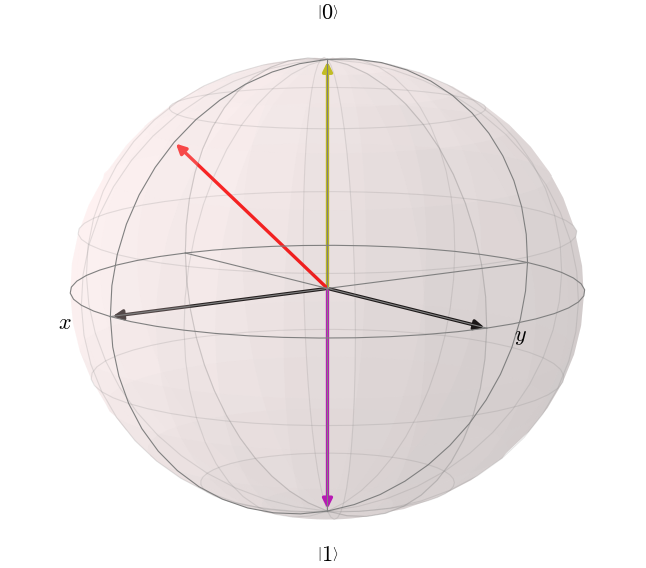
\includegraphics[scale=0.5]{img/3over4state.png}
       \caption{\label{fig:3over4}Simple binary classification problem of a quantum state}
\end{figure}

\begin{minipage}[c]{.49\textwidth}
    \begin{tabular}{| C{0.8cm} | C{1.7cm} |C{2cm}|}
      \toprule
      Qubit state & Vector representation & Class\\
      \midrule
       $\ket{0}$ & $\colvec{1\\0}$ & $\ket{0}$ (yellow)\\\midrule
       $\ket{1}$ & $\colvec{0\\1}$ & $\ket{1}$ (purple)\\\midrule
      \bottomrule
    \end{tabular}
        \label{tab:trainingset}
        \captionsetup{justification=raggedright, singlelinecheck=false}
    \captionof{table}{Training set}
\end{minipage}%%%%
\begin{minipage}[c][][b]{.49\textwidth}
\flushright
    \begin{tabular}{| C{2.7cm} | C{2.3cm} |C{2cm}|}
      \toprule
      Qubit state & Vector representation & Expected class\\
      \midrule
       $e^{-i\frac{\pi}{8}}\big[0.92388\ket{0} + 0.38268\ket{1}\big]$ & $e^{-i\frac{\pi}{8}}\colvec{0.92388\\0.38268}$ & $\ket{0}$ (yellow)\\\midrule
      \bottomrule
    \end{tabular}
        \label{tab:inputvectors}
        \captionsetup{justification=raggedleft, singlelinecheck=false}
    \captionof{table}{Input vector}
\end{minipage}

\subsubsection{Initial state preparation}
\label{subsubsubsec:initialstatepreparation}

The first step towards an actual implementation of this problem is to prepare the initial quantum state $\ket{\psi_0}$ previously defined in Equ.~\ref{equ:ampinitial} to be of the form,
\begin{equation}
\label{equ:ampinitial2}
\ket{\psi_0} = \frac{1}{\sqrt{2M}}\sum_{m=1}^{M} (\textcolor{emerald}{\ket{0}}\ket{\textcolor{red}{\Psi_{x}}}+\textcolor{emerald}{\ket{1}}\ket{\textcolor{darkyellow}{\Psi}_{\textcolor{purple}{t^{m}}}})\ket{c^{m}}\ket{m}
\end{equation}

where in the case of the selected classification problem:
\begin{align} 
\label{equ:vectordefs}
&\ket{\textcolor{red}{\Psi_{x}}} = e^{-i\frac{\pi}{8}}\big[0.92388\ket{0} + 0.38268\ket{1}\big]\\
&\ket{\textcolor{darkyellow}{\Psi_{t^{1}}}} = \ket{0} \\
&\ket{\textcolor{purple}{\Psi_{t^{2}}}} = \ket{1}
\end{align}
 
Since there are only two training vectors the index $m$ in Equ.~\ref{equ:ampinitial2} only takes the values 1 and 2. However, the $m$ qubit can only take binary values such that we need to redefine $1\rightarrow 0$ and $2\rightarrow 1$. With this observation, the required number of qubits can be deduced from Equ.~\ref{equ:ampinitial2}: one ancilla, one qubit for input and training vectors, one class qubit and one $m$ qubit making a total of four qubits. In the subsequent discussion the quantum state of the IBM QC in the $i^{th}$ step will be denoted $\ket{\chi_i}$. Since all qubits in the IBM Quantum Composer are initialized in state \0 the initial state $\ket{\chi_0}$ is simply,
\begin{equation}
\ket{\chi_0} = \ket{a}\ket{d}\ket{c}\ket{m} = \ket{0}\ket{0}\ket{0}\ket{0}
\end{equation}

where $a$ stands for ancilla, $d$ for data, $c$ for class and $m$ for the $m$ qubit. The sum over $m$ is introduced by simply acting an H gate on the $m$ qubit:
\begin{equation}
\ket{\chi_1} = (\mathbb{1} \otimes \mathbb{1} \otimes \mathbb{1} \otimes H)\ket{0}\ket{0}\ket{0}\ket{0} = \frac{1}{\sqrt{2}} \sum_{m=0}^1 \ket{0}\ket{0}\ket{0}\ket{m}
\end{equation}
%ADD CIRCUIT REPRESENTATION?

Using another H gate, the ancilla qubit is put in superposition:
\begin{equation}
\ket{\chi_2} = (H \otimes \mathbb{1} \otimes \mathbb{1} \otimes \mathbb{1})\ket{\chi_1} = \frac{1}{2} \sum_{m=0}^1 \ket{0}\ket{0}\ket{0}\ket{m} + \ket{1}\ket{0}\ket{0}\ket{m} = \frac{1}{2} \sum_{m=0}^1 \big[ \ket{0}\ket{0} + \ket{1}\ket{0}\big] \ket{0}\ket{m}
\end{equation}
%ADD CIRCUIT REPRESENTATION?

Next, the input vector $\ket{\textcolor{red}{\Psi_{x}}}$ should be loaded into the quantum state by means of a yet unknown gate sequence $GS$ such that the state is described by,

\begin{align}
\label{equ:chi3}
\ket{\chi_3} &= GS \ket{\chi_2} = \frac{1}{2} \sum_{m=0}^1 \big[ \ket{0}\ket{\textcolor{red}{\Psi_{x}}} + \ket{1}\ket{0}\big] \ket{0}\ket{m}\notag\\
&= \frac{1}{2} \sum_{m=0}^1 \Big[ \ket{0}\textcolor{red}{e^{-i\frac{\pi}{8}}\big[0.92388\ket{0} + 0.38268\ket{1}\big]} + \ket{1}\ket{0}\Big] \ket{0}\ket{m}
\end{align}

By looking closely at Fig.~\ref{fig:3over4} one can deduce that the red input vector can be reached by simply rotating the \0 vector by an angle of $\frac{\pi}{4}$ around the y-axis. A y-rotation by an arbitrary angle $\vartheta$ can be achieved with the rotation operator $R_y(\vartheta)$. As described by \citeA{nielsen2010quantum}, $R_y(\vartheta)$ can be represented as a unitary 2x2 matrix and is obtained from exponentiating the Y gate as shown in Equ.~\ref{equ:rydef}.

\begin{equation}
\label{equ:rydef}
R_y(\vartheta) = e^{-i\vartheta\frac{Y}{2}} = \text{cos}\frac{\vartheta}{2}\mathbb{1} - i\text{sin}\frac{\vartheta}{2}Y = \begin{pmatrix}
\text{cos}\frac{\vartheta}{2} & -\text{sin}\frac{\vartheta}{2} \\
\text{sin}\frac{\vartheta}{2} & \text{cos}\frac{\vartheta}{2}
\end{pmatrix}
\end{equation}

At this point, note that $R_y(\vartheta)$ is not an element of IBM's universal gate set. The problem of how to implement $R_y(\vartheta)$ on the IBM QC will be addressed later. For now, suppose $R_y(\frac{\pi}{4})$ can be implemented. Acting this gate on the data qubit in $\ket{\chi_2}$ yields the expression

\begin{equation}
(\mathbb{1} \otimes R_y(\frac{\pi}{4}) \otimes \mathbb{1} \otimes \mathbb{1})\ket{\chi_2} = \frac{1}{2} \sum_{m=0}^1 \big[ \ket{0}\ket{\textcolor{red}{\Psi_{x}}} + \ket{1}\ket{\textcolor{red}{\Psi_{x}}}\big] \ket{0}\ket{m}
\end{equation}

This, however, is not the desired state $\ket{\chi_3}$ defined in Equ.~\ref{equ:chi3} since the input vector $\ket{\textcolor{red}{\Psi_{x}}}$ should only be entangled with the \0 state of the ancilla. To achieve this type of entanglement the controlled version of the y-rotation gate, $CR_y(\frac{\pi}{4})(c,t)$, is required. When applying it using the $a$ qubit as control and the $d$ qubit as target the input vector will be entangled with the \1 state of the ancilla. Flipping the $a$ qubit with an X gate moves the input vector to the \0 state of the ancilla. Hence, the desired state $\ket{\chi_3}$ is obtained by applying the following gate sequence $GS$:
\begin{equation}
\label{equ:gs}
GS = (X \otimes \mathbb{1} \otimes \mathbb{1} \otimes \mathbb{1}) (CR_y(\frac{\pi}{4})(a,d) \otimes \mathbb{1} \otimes \mathbb{1}) \\
\end{equation}
subbing into Equ.~\ref{equ:chi3}:
\begin{align}
\label{equ:chi3prepared}
\ket{\chi_3} &=  GS \ket{\chi_2} = (X \otimes \mathbb{1} \otimes \mathbb{1} \otimes \mathbb{1}) (CR_y(\frac{\pi}{4})(a,d) \otimes \mathbb{1} \otimes \mathbb{1}) \ket{\chi_2}\notag\\
&= (X \otimes \mathbb{1} \otimes \mathbb{1} \otimes \mathbb{1}) \Big[\frac{1}{2} \sum_{m=0}^1 \big[\ket{0}\ket{0} + \ket{1}\ket{\textcolor{red}{\Psi_{x}}}\big] \ket{0}\ket{m}\Big]\notag\\
&= \frac{1}{2} \sum_{m=0}^1 \Big[ \ket{0}\ket{\textcolor{red}{\Psi_{x}}} + \ket{1}\ket{0}\Big] \ket{0}\ket{m}
\end{align}

It is important to note that also $CR_y(\frac{\pi}{4})(c,t)$ is not an element of IBM's universal gate set. Its implementation on the IBM QC will be discussed in the next subsection.

The next step is to entangle the first training vector $\ket{\textcolor{darkyellow}{\Psi_{t^{0}}}}$  with the \1 state of the ancilla and the \0 state of the $m$ qubit. Additionally, the second training vector $\ket{\textcolor{purple}{\Psi_{t^{1}}}}$ should be entangled with the \1 states of the ancilla and the $m$ qubit. Note that $\ket{\textcolor{darkyellow}{\Psi_{t^{1}}}}$ and $\ket{\textcolor{purple}{\Psi_{t^{2}}}}$ defined in Equ.~\ref{equ:vectordefs} were redefined to $\ket{\textcolor{darkyellow}{\Psi_{t^{0}}}}$ and $\ket{\textcolor{purple}{\Psi_{t^{1}}}}$ respectively. Expanding the sum in Equ.~\ref{equ:chi3prepared} demonstrates that $\ket{\textcolor{darkyellow}{\Psi_{t^{0}}}} = \ket{0}$ is already at its desired place:

\begin{align}
\label{equ:chi3expanded}
\ket{\chi_3} &= \frac{1}{2}\Big[ \big[\ket{0}\ket{\textcolor{red}{\Psi_{x}}} + \ket{1}\ket{0}\big] \ket{0}\ket{0} + \big[ \ket{0}\ket{\textcolor{red}{\Psi_{x}}} + \ket{1}\ket{0}\big] \ket{0}\ket{1}\Big]\notag\\
&= \frac{1}{2}\Big[ \big[\ket{0}\ket{\textcolor{red}{\Psi_{x}}} + \ket{1}\ket{\textcolor{darkyellow}{\Psi_{t^{0}}}}\big] \ket{0}\ket{0} + \big[ \ket{0}\ket{\textcolor{red}{\Psi_{x}}} + \ket{1}\ket{0}\big] \ket{0}\ket{1}\Big]
\end{align}

In order to entangle $\ket{\textcolor{purple}{\Psi_{t^{1}}}}$ with the \1 states of the ancilla and $m$ qubit a Toffoli (CCNOT) gate needs to be implemented. Using the ancilla ($a$) and $m$ qubit as controls and choosing the data ($d$) qubit as target one obtains the following state:

\begin{align}
\label{equ:chi4}
\ket{\chi_4} &= CCNOT(a,m,d)\ket{\chi_3}\notag\\
&= \frac{1}{2}\Big[ \big[\ket{0}\ket{\textcolor{red}{\Psi_{x}}} + \ket{1}\ket{\textcolor{darkyellow}{\Psi_{t^{0}}}}\big] \ket{0}\ket{0} + \big[ \ket{0}\ket{\textcolor{red}{\Psi_{x}}} + \ket{1}\ket{1}\big] \ket{0}\ket{1}\Big]\notag\\
&= \frac{1}{2}\Big[ \big[\ket{0}\ket{\textcolor{red}{\Psi_{x}}} + \ket{1}\ket{\textcolor{darkyellow}{\Psi_{t^{0}}}}\big] \ket{0}\ket{0} + \big[ \ket{0}\ket{\textcolor{red}{\Psi_{x}}} + \ket{1}\ket{\textcolor{purple}{\Psi_{t^{1}}}}\big] \ket{0}\ket{1}\Big]
\end{align}

The class qubit for the first training vector is already in the correct \0 state. Note again that also the CCNOT gate is not element of IBM's universal gate set which will be addressed later.

It remains to flip the class qubit for the second training vector by applying a CNOT gate using the $d$ qubit as control and the class($c$) qubit as target. The resulting state is then given by,

\begin{align}
\label{equ:chi5}
\ket{\chi_5} &= CNOT(d,c)\ket{\chi_4}\notag\\
&= \frac{1}{2}\Big[ \big[\ket{0}\ket{\textcolor{red}{\Psi_{x}}} + \ket{1}\ket{\textcolor{darkyellow}{\Psi_{t^{0}}}}\big] \ket{\textcolor{darkyellow}{0}}\ket{0} + \big[ \ket{0}\ket{\textcolor{red}{\Psi_{x}}} + \ket{1}\ket{\textcolor{purple}{\Psi_{t^{1}}}}\big] \ket{\textcolor{purple}{1}}\ket{1}\Big]
\end{align}

and can be rewritten as:

\begin{align}
\label{equ:chi5psi0}
\ket{\chi_5} &= \frac{1}{2} \sum_{m=1}^{2} \big[\ket{0}\ket{\textcolor{red}{\Psi_{x}}} + \ket{1}\ket{\textcolor{darkyellow}{\Psi_{t^{0}}}}\big] + \big[ \ket{0}\ket{\textcolor{red}{\Psi_{x}}} + \ket{1}\ket{\textcolor{purple}{\Psi_{t^{1}}}}\big]\ket{c^{m}}\ket{m}\notag\\
&= \frac{1}{2} \sum_{m=1}^{2} \big[\ket{0}\ket{\textcolor{red}{\Psi_{x}}} + \ket{1}\ket{\textcolor{darkyellow}{\Psi_{\textcolor{purple}{t^{m}}}}}\big]\ket{c^{m}}\ket{m}
\end{align}

When comparing Equ.~\ref{equ:chi5psi0} to $\ket{\psi_0}$ in Equ.~\ref{equ:ampinitial} it becomes clear that $\ket{\chi_5}$ is in the form of the desired initial quantum state $\ket{\psi_0}$. The quantum state preparation is therefore theoretically completed.

\subsubsection{Decomposition of a controlled-U gate}
\label{subsubsubsec:controlledugate}

To implement the quantum state preparation on the IBM QC, it remains to find a way of realizing the controlled y-rotation $CR_y(\frac{\pi}{4})(c,t)$ using only the ten gates from IBM's universal gate set. In their book \citeA{nielsen2010quantum} describe how a controlled U (CU) gate can be decomposed into a sequence of CNOT and single qubit gates. Thereby, U can be any unitary single-qubit gate. A CU gate is then defined as:
\begin{equation}
CU = \begin{pmatrix}
 \mathbb{1} & 0 \\ 
 0 & U
 \end{pmatrix}
\end{equation}

Most of the time the CU gate cannot be implemented directly since it is not element of the universal gate set at hand and it has to be realized through larger quantum circuits. Fig.~\ref{img:cudecomposition} shows the decomposition described by \citeA{nielsen2010quantum} into two CNOTs, three unitary single-qubit gates $A,B,C$ and a phase-adjusting matrix which will be denoted $P$ of the form:
\begin{equation}
P = \begin{pmatrix}
 1 & 0 \\ 
 0 & e^{i\alpha}
 \end{pmatrix}
\end{equation}

\begin{figure}[ht]
   \centering
   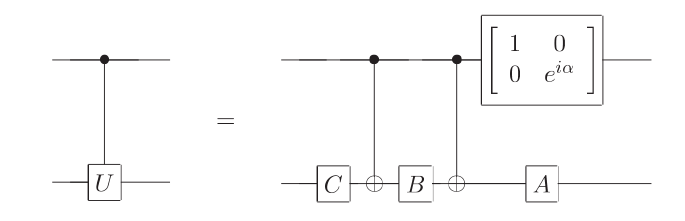
\includegraphics[width=0.7\textwidth]{img/controlledudecomp.png}
   \caption[]{Circuit decomposition of controlled-U quantum gate.\footnotemark[14]}
   \label{img:cudecomposition}
\end{figure}

\footnotetext[14]{Reprinted from Michael A. Nielsen and Isaac L. Chuang. Quantum Computation and Quantum Information. Cambridge University Press, 2000. Copyright 2010 by Nielsen \& Chuang.}

The idea of this decomposition is that when the control qubit (top qubit in Fig.~\ref{img:cudecomposition}) is \0 the gate combination $ABC$ is applied to the target qubit (bottom qubit in Fig.~\ref{img:cudecomposition}) and has to equal the identity gate:

\begin{equation}
\label{equ:abcidentity}
ABC = \mathbb{1}
\end{equation}

If and only if the control qubit is \1 then the gate sequence $e^{i\alpha}AXBXC$ is applied to the target. Since the goal is to apply the unitary U to the target qubit the following equation must be satified:
\begin{equation}
\label{equ:UAXBXC}
e^{i\alpha}AXBXC = U
\end{equation}

\citeA{nielsen2010quantum} make the following choices for the unitary gates $A,B,C$:

\begin{align}\label{equ:abc}
A &=  R_z(\beta)R_y(\frac{\gamma}{2})\\
B &= R_y(-\frac{\gamma}{2})R_z(-\frac{\delta+\beta}{2})\\
C &= R_z(\frac{\delta-\beta}{2})
\end{align}

where $R_z(\varrho)$ is the general rotation gate about the z-axis of the Bloch sphere. Similary to the $R_y(\vartheta)$ gate it can be obtained by exponentiating the Z gate as shown below in Equ.~\ref{equ:rzdef}.

\begin{equation}
\label{equ:rzdef}
R_z(\varrho) = e^{-i\varrho\frac{Z}{2}} = \text{cos}\frac{\varrho}{2} \mathbb{1}- i\text{sin}\frac{\varrho}{2}Z = \begin{pmatrix}
e^{-i\frac{\varrho}{2}} & 0 \\
0 & e^{i\frac{\varrho}{2}}
\end{pmatrix}
\end{equation}

When subbing the expressions for $A,B,C$ from Equ.~\ref{equ:abc} into Equ.~\ref{equ:abcidentity} one will indeed obtain the identity operation (proof omitted). These choices of $A,B,C$ are also a solution to Equ.~\ref{equ:UAXBXC}. Subbing into Equ.~\ref{equ:UAXBXC} leads to the following expression for matrix $U$:

\begin{equation}
\label{equ:udecompdef}
U = \begin{pmatrix}
 e^{i(\alpha-\frac{\beta}{2}-\frac{\delta}{2})}\cos{\frac{\gamma}{2}} & -e^{i(\alpha-\frac{\beta}{2}+\frac{\delta}{2})}\sin{\frac{\gamma}{2}} \\ 
e^{i(\alpha+\frac{\beta}{2}-\frac{\delta}{2})}\sin{\frac{\gamma}{2}} & e^{i(\alpha+\frac{\beta}{2}+\frac{\delta}{2})}\cos{\frac{\gamma}{2}}
 \end{pmatrix}
\end{equation}
%Furthermore, \citeA{nielsen2010quantum} show that any unitary matrix U can be decomposed as,
%\begin{equation}
%\label{equ:URzRyRz}
%U = e^{i\alpha}R_z(\beta)R_y(\gamma)R_z(\delta)
%\end{equation}
%\begin{equation}
%\label{equ:UAXBXC}
%e^{i\alpha}AR_x(\pi)BR_x(\pi)C = U
%\end{equation}

To decompose $CR_y(\frac{\pi}{4})$, one simply chooses $U = R_y(\frac{\pi}{4})$. Subbing $\vartheta = \frac{\pi}{4}$ into Equ.~\ref{equ:rydef} the matrix representation of $R_y(\frac{\pi}{4})$ is obtained:

\begin{equation}
U = R_y(\frac{\pi}{4}) = \begin{pmatrix}
\text{cos}\frac{\pi}{8} & -\text{sin}\frac{\pi}{8} \\
\text{sin}\frac{\pi}{8} & \text{cos}\frac{\pi}{8}
\end{pmatrix}
\end{equation}

Subbing this expression for $U$ into Equ.~\ref{equ:udecompdef} leads to:

\begin{equation}
\label{equ:udecompsubbed}
U = \begin{pmatrix}
\text{cos}\frac{\pi}{8} & -\text{sin}\frac{\pi}{8} \\
\text{sin}\frac{\pi}{8} & \text{cos}\frac{\pi}{8}
\end{pmatrix} = \begin{pmatrix}
 e^{i(\alpha-\frac{\beta}{2}-\frac{\delta}{2})}\cos{\frac{\gamma}{2}} & -e^{i(\alpha-\frac{\beta}{2}+\frac{\delta}{2})}\sin{\frac{\gamma}{2}} \\ 
e^{i(\alpha+\frac{\beta}{2}-\frac{\delta}{2})}\sin{\frac{\gamma}{2}} & e^{i(\alpha+\frac{\beta}{2}+\frac{\delta}{2})}\cos{\frac{\gamma}{2}}
 \end{pmatrix}
\end{equation}

When setting the expressions for the respective matrix entries in Equ.~\ref{equ:udecompsubbed} equal, the following system of non-linear complex equations is obtained :

\begin{align}
\label{equ:nlsystem}
\text{cos}\frac{\pi}{8} &= e^{i(\alpha-\frac{\beta}{2}-\frac{\delta}{2})}\cos{\frac{\gamma}{2}}\\
-\text{sin}\frac{\pi}{8} &= -e^{i(\alpha-\frac{\beta}{2}+\frac{\delta}{2})}\sin{\frac{\gamma}{2}}  \\
\text{sin}\frac{\pi}{8} &= e^{i(\alpha+\frac{\beta}{2}-\frac{\delta}{2})}\sin{\frac{\gamma}{2}}\\
\text{cos}\frac{\pi}{8} &= e^{i(\alpha+\frac{\beta}{2}+\frac{\delta}{2})}\cos{\frac{\gamma}{2}}\\
\end{align}

This is a system of four non-linear complex equations with four unknowns. In order to solve for the parameters $\alpha,\beta,\gamma$ and $\delta$ one can use any root finding algorithm for non-linear equations such as Secant or Newton's method. Using Newton's method the solutions are found to be:
\begin{equation}
\alpha =  \pi; \quad 
\beta = 2\pi;\quad 
\delta = \frac{7}{8}\pi;\quad 
\gamma = 0
\end{equation}

Subbing these parameters into the expressions for $A,B$ and $C$ defined in Equ.~\ref{equ:abc} yields,

\begin{align}
\label{equ:abcsubbed1}
A \quad= \quad R_z(\beta)R_y(\frac{\gamma}{2})\quad =& \quad R_z(2\pi) \quad = \quad \textcolor{emerald}{\mathbb{1}} \\
\label{equ:abcsubbed2}
B\quad =\quad R_y(-\frac{\gamma}{2})R_z(-\frac{\delta+\beta}{2})\quad =& \quad R_z(-\frac{23}{16}\pi) \quad= \quad \textcolor{red}{?}  \\
\label{equ:abcsubbed3}
C \quad=\quad R_z(\frac{\delta-\beta}{2})\quad =& \quad R_z(-\frac{9}{16}\pi) \quad= \quad \textcolor{red}{?} \\
\label{equ:abcsubbed4}
P\quad =\quad \begin{pmatrix} 1&0\cr0&e^{i\alpha} \end{pmatrix}\quad=& \quad \begin{pmatrix} 1&0\cr0&e^{i\pi} \end{pmatrix}\quad= \quad \textcolor{emerald}{Z}
\end{align}

Quantum gate $A$ is just equal to the identity gate which certainly is element of IBM's universal gate set. The phase-adjusting gate $P$ is equal to the Z gate that also is within IBM's gate set. Only gates $B$ and $C$ result in more complex z-rotations of $-\frac{23}{16}\pi$ and $-\frac{9}{16}\pi$ radians respectively. Unfortunately, these quantum gates are not found in IBM's gate set as indicated by the red question marks in Equ.~\ref{equ:abcsubbed2} and \ref{equ:abcsubbed3}.

\subsubsection{The Solovay-Kitaev theorem}
\label{subsubsubsec:solovaykitaev}

An important theorem in quantum information is the Solovay-Kitaev theorem first proposed by Robert M. Solovay and later published by \citeA{kitaev1995quantum}. It will be used to decompose the quantum gates $B$ and $C$ into a sequence of quantum gates from IBM's universal gate set.

At this point, it is important to remember that any universal quantum gate set is a dense subset of the special unitary group $SU(2)$ as previously defined in Section~\ref{subsubsec:qubits}.

\begin{redbox}
\textbf{Theorem: Solovay-Kitaev theorem}\\
\newline
Let $G$ be a universal quantum set $G$ consisting of quantum gates from $SU(2)$ and let $\epsilon > 0$ be a desired accuracy. Then there is a constant $b$ such that for any single-qubit gate $W \in SU(2)$ there exists a
finite gate sequence $\tilde{G}$ of gates from the set $G$ of length $O(log^b (1/\epsilon))$ such that $d(W, \tilde{G}) < \epsilon$. In their proof, \citeA{dawson2005solovay} show that $b \approx 3.97$.\\
\newline
In other words, given a set of single-qubit quantum gates which is a dense subset of $SU(2)$, then the Solovay-Kitaev theorem guarantees that this set will quickly fill $SU(2)$.
\cite{dawson2005solovay}.
\end{redbox}

The Solovay-Kitaev theorem is important because it proofs that given any universal gate set it is possible to obtain good approximations to any desired single-qubit gate $W$. In their paper, \citeA{dawson2005solovay} describe how to design an algorithm implementing the Solovay-Kitaev theorem. Unfortunately, the Solovay-Kitaev algorithm needs to be implemented on a classical computer which adds to the overall time complexity of the quantum compiling process as will be shown later. For this thesis, the open-source software package 'Quantum Compiler, v0.03'\footnotemark[15] developed in Python by Paul Pham was used to run the Solovay-Kitaev algorithm described by \citeA{dawson2005solovay}. This software package compares different gate approximations to the desired gate by a new distance metric called Fowler distance.

\footnotetext[15]{The software package 'Quantum Compiler, v0.03' by Paul Pham can be downloaded from \url{https://sourceforge.net/projects/quantumcompiler/files/v0.03/}.}

\begin{redbox}
\textbf{Definition: Fowler distance}\\
\newline
When approximating a unitary gate $W$ with a gate sequence yielding another unitary gate $W_{approx}$ it is important to quantify how 'close' the action of $W_{approx}$ is to $W$. The Fowler distance makes use of the matrix representations of $W$ and $W_{approx}$ and is defined by \citeA{booth2012quantum} as:
\begin{equation}
d(W,W_{approx}) = \sqrt{\frac{2-\mid tr(W\cdot W_{approx}^\dagger)\mid}{2}}
\end{equation}

In contrast to $W$, $W_{approx}$ might introduce a shift in the global phase of the quantum state it is acting on. However, since the global phase of a quantum state is immeasurable in experiment it can be neglected. As a result, the Fowler distance is defined in such a way that possible global phase differences are ignored.
\end{redbox}

Subsequently, the desired gates $B = R_z(-\frac{23}{16}\pi)$ and $C = R_z(-\frac{9}{16}\pi)$ where decomposed using the Solovay-Kitaev algorithm. Fig.~\ref{fig:skresultplot} shows a plot visualizing how the Fowler distance depends on the number of gates in the approximating gate sequence $W_{approx}$. The number of gates in the approximating gate sequence is also called \emph{gate count}. The plot clearly shows an exponential increase in the gate count for decreasing Fowler distance. For example, 146 gates suffice to achieve $d(W_{approx},R_z(-\frac{9}{16}\pi)) = 0.04389$. Yet, already 17,838 gates are required to reduce the Fowler distance to $d(W_{approx},R_z(-\frac{9}{16}\pi)) = 0.01008$.

\begin{figure}[H]
\centering
    \begin{tikzpicture}[scale=1]
\begin{axis}[xlabel={Gate count},ylabel={Fowler distance [$d(U,U_{approx})$]}]

% Graph column 2 versus column 0
\addplot table[x index=1,y index=0,col sep=comma] {datax.dat};
\addlegendentry{$R_z(-\frac{9}{16}\pi)$}% y index+1 since humans count from 1

% Graph column 1 versus column 0    
\addplot table[x index=5,y index=4,col sep=comma] {datax.dat};
\addlegendentry{$R_z(-\frac{23}{16}\pi)$}

\end{axis}
\end{tikzpicture}
\caption{Fowler distance plotted against the required gate count for quantum gates $B = R_z(-\frac{23}{16}\pi)$ and $C = R_z(-\frac{9}{16}\pi)$ }
\label{fig:skresultplot}
  \end{figure}
  
Fowler distance is best understood with a visual example using the gate $B = R_z(-\frac{23}{16}\pi)$. Acting the desired gate $B$ on the state $\ket{\psi} = \frac{\ket{0} + \ket{1}}{\sqrt{2}}$ (black vector in Fig.~\ref{fig:bloch23over16}) results in the purple Bloch vector $\vec{b}$ shown in Fig.~\ref{fig:bloch23over16}.

\begin{figure}[H]
\centering
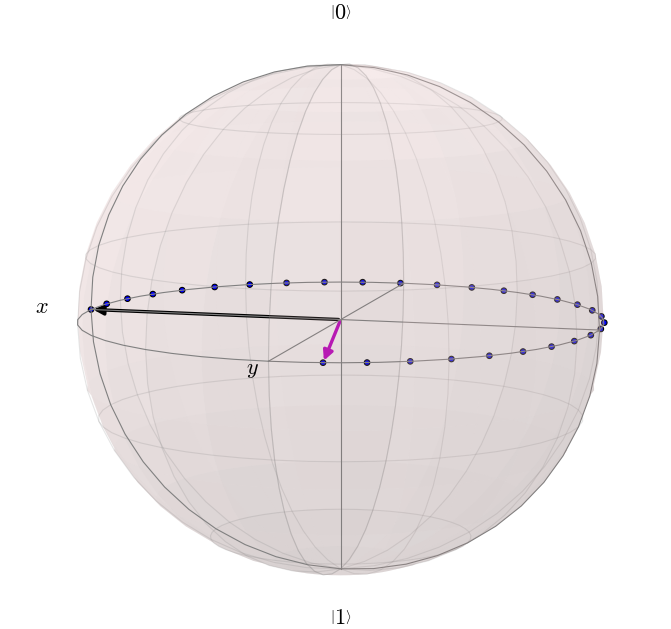
\includegraphics[scale=0.4]{img/bloch23over16.png}
\caption{\label{fig:bloch23over16} Action of $B = R_z(-\frac{23}{16}\pi)$ on the state $\ket{\psi} = \frac{\ket{0} + \ket{1}}{\sqrt{2}}$}
\end{figure}

Fig.~\ref{fig:fowlerdistances} shows the action of four different approximating gate sequences $B_{approx,1}$, $B_{approx,2}$, $B_{approx,3}$, $B_{approx,4}$ on the state $\ket{\psi} = \frac{\ket{0} + \ket{1}}{\sqrt{2}}$. Gate sequence $B_{approx,1}$ consists of 25 gates and is a Fowler distance of $d = 0.15165$ away from $B$. The resulting state vector is coloured green in Fig.~\ref{fig:fowlerdistances}. The green vector lies above the Bloch equator and is relatively far away from the desired vector $\vec{b}$ in Fig.~\ref{fig:bloch23over16}. With 109 gates, $B_{approx,2}$ yields a Fowler distance of $d = 0.10722$ resulting in the blue vector. It is also found below the Bloch equator and still relatively far from $\vec{b}$. Using $B_{approx,3}$ the Fowler distance drops to $d = 0.02086$ leading to the yellow vector in  Fig.~\ref{fig:fowlerdistances}. This vector is almost on the Bloch equator and relatively close to $\vec{b}$ implying that $B_{approx,3}$ is a good approximation of $B$. However, $B_{approx,3}$ already requires the implementation of 2,997 single-qubit gates. The purple vector from Fig.~\ref{fig:bloch23over16} is also plotted in Fig.~\ref{fig:fowlerdistances} but is not visible since the red vector with $d = 0.00158$ constitutes a very good approximation to the desired state $\vec{b}$.  The red vector is the result of the action of $B_{approx,4}$ which, unfortunately, needs 370,813 gates to achieve such a small Fowler distance. Hereby, Gate $B$ was used as an example but such an exponential increase in the gate count is observed for any quantum gate $W$ when applying the Solovay-Kitaev algorithm \cite{dawson2005solovay}.

\begin{minipage}[c]{.8\textwidth}
	%\vspace{-20mm}
	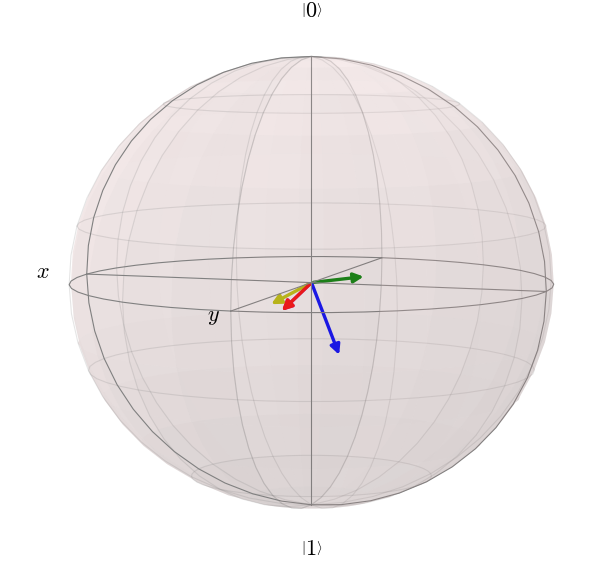
\includegraphics[height=0.8\textwidth]{img/fowlerdistances.png}
       \captionsetup{justification=raggedright, singlelinecheck=false}
       \captionof{figure}{\label{fig:fowlerdistances}Various Fowler distances visualized on Bloch sphere }
\end{minipage}%%%%%
\begin{minipage}[c]{.2\textwidth}
\begin{equation}
\textcolor{emerald}{d = 0.15165} \notag
\end{equation}
\begin{equation}
\textcolor{blue}{d = 0.10722} \notag
\end{equation}
\begin{equation}
\textcolor{darkyellow}{d = 0.02086} \notag
\end{equation}
\begin{equation}
\textcolor{red}{d = 0.00158} \notag
\end{equation}

\end{minipage}

Implementing any quantum gate $D$ inevitably takes some time $t$ since it involves the use of hardware components e.g. targeting a specific electron with a laser pulse. Based on IBM's single-qubit and CNOT gate times described in Section~\ref{subsec:ibmqc} the total execution time of twelve different gate sequences, approximating $B = R_z(-\frac{23}{16}\pi)$ and $C = R_z(-\frac{9}{16}\pi)$ to different Fowler distances, were calculated. The results can be seen in Table~\ref{tab:sktimes}. Keeping in mind that in the best case, the maximum decoherence time of a qubit in IBM's QC is \SI{112.4}{\micro\second} most gate sequences are too long for an IBM implementation (coloured red in Table~\ref{tab:sktimes}). Feasible execution times are marked green in Table~\ref{tab:sktimes}. However, decoherence is not the only limiting factor since IBM only allows for 39 gates and one measurement gate. But even when selecting the smallest sequences of 25 gates for $B$ and 16 gates for $C$, the total gate count is 41 which is two gates more than the allowed gate count of the IBM Quantum Composer. Furthermore, the approximating gate sequences of $B$ and $C$ are not the only gates needed to prepare the initial quantum state and execute the akNN algorithm. Unfortunately, this makes an actual implementation of this particular classification problem on IBM's QC impossible.

%Thus, the only possibility would be to select the sequence of 25 gates for $B$ and the sequence of 16 gates for $C$ at the cost of relatively large Fowler distances. This, however, still sums up to 41 gates which is two gates more than the allowed gate count of the IBM Quantum Composer. 

\begin{table}[H]
\centering
    \begin{tabular}{c| c |c |c }
      \toprule
      Approx. Gate & Fowler distance & Gate count & Execution time\\
      \midrule
      $R_z(-\frac{23}{16}\pi)$ & 0.15165 & 25 & \textcolor{emerald}{$\sim$\SI{3}{\micro\second}}\\
       & 0.10722 & 109 & \textcolor{emerald}{$\sim$\SI{14}{\micro\second}}\\
       & 0.02086 & 2,997 & \textcolor{red}{$\sim$\SI{390}{\micro\second}}\\
       & 0.01494 & 14,721 & \textcolor{red}{$\sim$\SI{1914}{\micro\second}}\\
       & 0.003327 & 74,009 & \textcolor{red}{$\sim$\SI{9621}{\micro\second}}\\
       & 0.001578 & 370,813 & \textcolor{red}{$\sim$\SI{48206}{\micro\second}}\\
       \midrule
      $R_z(-\frac{9}{16}\pi)$ & 0.28390 & 16 & \textcolor{emerald}{$\sim$\SI{2}{\micro\second}}\\
       & 0.04389 & 146 & \textcolor{emerald}{$\sim$\SI{18}{\micro\second}}\\
       & 0.049511 & 728 & \textcolor{emerald}{$\sim$\SI{87}{\micro\second}}\\
       & 0.02823 & 3,622 & \textcolor{red}{$\sim$\SI{435}{\micro\second}}\\
       & 0.01008 & 17,838 & \textcolor{red}{$\sim$\SI{2141}{\micro\second}}\\
       & 0.00156 & 444,646 & \textcolor{red}{$\sim$\SI{53358}{\micro\second}}\\
      \bottomrule
      \bottomrule
    \end{tabular}
    \caption{\label{tab:sktimes} Results of the Solovay-Kitaev algorithm for decomposition of $B = R_z(-\frac{23}{16}\pi)$ and $C = R_z(-\frac{9}{16}\pi)$}
  \end{table}
  
To complete the quantum compiling, assume that gates $B$ and $C$ could somehow be implemented with shorter gate sequences. It remains to decompose the Toffoli gate that was required to 'load' the second training pattern $\ket{\textcolor{purple}{\Psi_{t^{1}}}}$ into the quantum state $\ket{\chi_4}$ as shown in Equ.~\ref{equ:chi4}.

\subsubsection{Toffoli Gate Decomposition}
\label{subsubsubsec:toffoli}

The Toffoli or CCNOT gate can be decomposed into CNOT and single-qubit gates in several ways. In their book,\citeA{nielsen2010quantum} describe the decomposition into six CNOTs and nine single-qubit gates; two H gates, three T and three T$^\dagger$ gates. See Fig.~\ref{img:toffolidecomp} for the corresponding circuit diagram. This decomposition does not require any further compiling work since all involved gates are elements of IBM's universal gate set.

\begin{figure}[!ht]
       \centering
       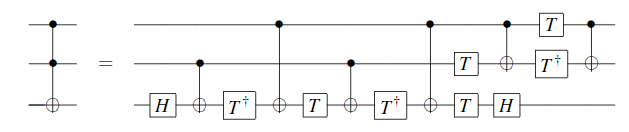
\includegraphics[scale=0.5]{img/toffolidecomposition.png}
       \caption[]{\label{img:toffolidecomp} Decomposition of a Toffoli gate into six CNOT and nine single-qubit gates\footnotemark[16]}
\end{figure}

\footnotetext[16]{Reprinted from Michael A. Nielsen and Isaac L. Chuang. Quantum Computation and Quantum Information. Cambridge University Press, 2000. Copyright 2010 by Nielsen \& Chuang.}

The Toffoli decomposition finalizes the compiling of the quantum state preparation into gates from IBM's gate set only. In summary, the compiled state preparation requires: 2 H gates applied to the ancilla and the $m$ qubit, the decomposed $CR_y(\frac{\pi}{4})$ gate (2 CNOTs, 1 Z gate, 1 $\mathbb{1}$ gate (can be neglected) \& a sequence of minimum 25 gates for $B$ and minimum 16 gates for $C$), 1 X gate to flip the ancilla (Equ.~\ref{equ:chi3prepared}), 1 decomposed Toffoli (6 CNOTs, 2 H gates, 3 T \& 3 T$^\dagger$ gates) to load the second training vector and 1 CNOT to flip the class qubit. Thus, the quantum state preparation was compiled into 9 CNOT and 53 single-qubit gates. The akNN algorithm only requires one additional H gate and two measurement gates (for ancilla and class qubit) leading to a total of 9 CNOT, 54 single-qubit gates and 2 measurement gates. However, even cleverly arranging these gates does not suffice to implement the algorithm within IBM's 40 gate slots. The full circuit diagram for the compiled state preparation and the akNN algorithm can be seen in Fig.~\ref{img:toffolidecomp}.

\begin{figure}[!ht]
       \centering
       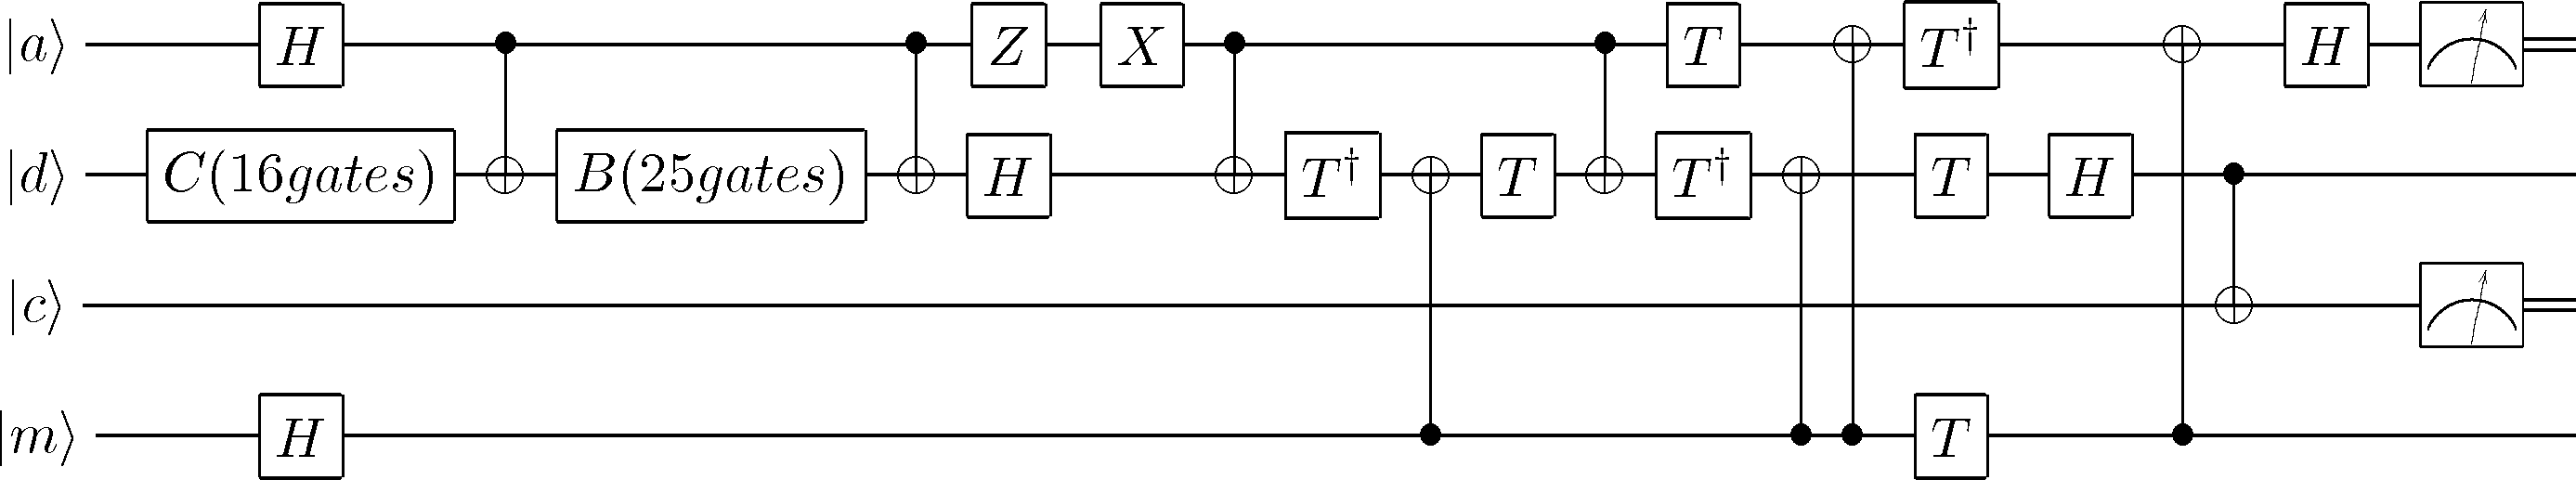
\includegraphics[width=\textwidth]{img/fullQKNN.png}
       \caption[]{\label{img:toffolidecomp} Compiled quantum circuit for implementing the akNN algorithm with the binary Bloch vector classification problem}
\end{figure}

%state preparation
%H Gate m qubit
%H Gate ancilla
%CR_y decomposed
%X Gate ancilla
%Toffoli(a,m,d)
%CNOT(d,c)

%algorithm
%H ancilla
%CM ancilla
%M class

%Final circuit diagram showing the compile state preparation + akNN algorithm steps

\begin{greenbox}
\textbf{Complexity analysis including quantum compiling steps}\\
\newline
The akNN algorithm itself was found to run in constant time $\mathcal{O}(\frac{1}{Prob(CM)})$. However, to determine the overall algorithmic complexity all steps required to prepare the initial quantum state $\ket{\psi_0}$ from Equ.~\ref{equ:ampinitial} need to be included. The decomposition of the $CR_y(\frac{\pi}{4})$ gate involved solving a system of non-linear equations by means of a root-finding algorithm. Any iterative root-finding algorithm e.g. Secant or Newton's method has a complexity of $\mathcal{O}(k)$ where $k$ is the number of root finding iterations. Furthermore, the Solovay-Kitaev algorithm was required to find two single-qubit gate sequences approximating the two gates $B = R_z(-\frac{23}{16}\pi)$ and $C = R_z(-\frac{9}{16}\pi)$. According to \citeA{dawson2005solovay} the Solovay-Kitaev algorithm has a complexity of $\mathcal{O}(m*log^{2.71}(\frac{m}{\epsilon}))$ for $\epsilon$-approximations of $m$ gates. Thus the total complexity is given by:
\begin{equation}
\mathcal{O}(\frac{1}{Prob(CM)})+\mathcal{O}(k)+\mathcal{O}(m*log^{2.71}(\frac{m}{\epsilon}))
\end{equation}
	
When adding algorithmic complexities only the most dominant term is considered relevant. Thus, the overall complexity including state preparation is found to be $\mathcal{O}(m*log^{2.71}(\frac{m}{\epsilon}))$.\\
\newline
In conclusion, due to the necessary quantum compiling steps the initial constant complexity of the akNN algorithm
\begin{equation}  
\mathcal{O}(\frac{1}{Prob(CM)})
\end{equation}
increased to a polylogarithmic complexity of
\begin{equation}
\mathcal{O}(m*log^{2.71}(\frac{m}{\epsilon}))
\end{equation}
dependening on the number of gates $m$ that need $\epsilon$-approximations by means of the Solovay-Kitaev algorithm.
\end{greenbox}

%All in all, it was shown that for this particular classification problem the constant complexity of the aKNN algorithm is dominated by the complexity of the quantum compiling. 

\subsection{Simulating the amplitude-based kNN algorithm}
\label{subsubsec:simulationamplitudeKNN}

Since the IBM Quantum Experience does not allow for an implementation, the aKNN algorithm was simulated in Liqui$\ket{}$ to determine the performance and the outcome of the algorithm. This section is subdivided into two parts: First, the classification of Bloch vectors described in the last section is simulated. Second, the aKNN algorithm is used to classify different Gaussian distributions constituting a slightly more complex classification task.

\subsubsection{Classification of Bloch vectors}
\label{subsubsubsec:classificationblochvectors}

The Bloch vector classification problem described in Section~\ref{subsubsec:implementationamplitudeKNN} was reconsidered and simulated in Liqui$\ket{}$ to determine if the algorithm yields the expected classification outcome. 

Section~\ref{subsubsec:implementationamplitudeKNN} pointed out that the implementation of the controlled y-rotation $CR_y(\frac{\pi}{4})$ was the main issue preventing an implementation within IBM's 40 gate slots. However, by specifying its matrix representation Liqui$\ket{}$ allows any unitary single- or multi-qubit gate to be defined within its programming framework. Therefore, $CR_y(\frac{\pi}{4})$ can be easily implemented in Liqui$\ket{}$. This enables to load the input vector specified in Table~\ref{tab:inputvectors} without having to decompose the controlled y-rotation gate and with no need for the Solovay-Kitaev algorithm. Due to this enormous simplification of the quantum state preparation routine, a second input vector was considered for simulation. Fig.~\ref{img:7over8} shows the new second input vector on the Bloch sphere. This new input vector can be obtained by rotating the \0 state by $\frac{\pi}{8}$ radians around the y-axis. The resulting new input data set is listed in Table~\ref{tab:inputvectors2}.

Table~\ref{tab:inputvectors2} shows that the probability of measuring the new input vector (ID=2) in state \0 is slightly higher than for the input vector with ID=1. This can also be seen visually when comparing Fig.~\ref{img:7over8} to Fig.~\ref{fig:3over4}. Lastly, the training data set listed in Table~\ref{tab:trainingset} was not altered for simulation.

\begin{table}[H]
\centering
\begin{tabular}{| C{0.5cm} | C{2.7cm} | C{2.3cm} |C{2cm}|}
      \toprule
      ID & Qubit state & Vector representation & Expected class\\
      \midrule
       1 & $e^{-i\frac{\pi}{8}}\big[0.92388\ket{0} + 0.38268\ket{1}\big]$ & $e^{-i\frac{\pi}{8}}\colvec{0.92388\\0.38268}$ & $\ket{0}$ (yellow)\\\midrule
       2 & $e^{-i\frac{\pi}{16}}\big[0.98079\ket{0} + 0.19509\ket{1}\big]$ & $e^{-i\frac{\pi}{16}}\colvec{0.98079\\0.19509}$ & $\ket{0}$ (yellow)\\\midrule
      \bottomrule
    \end{tabular}
    \caption{\label{tab:inputvectors2} Input data set II for the simulation of the aKNN algorithm. The data set consists of two different qubit states both lying in the z-x plane of the Bloch sphere.}
\end{table}

\begin{figure}[H]
       \centering
       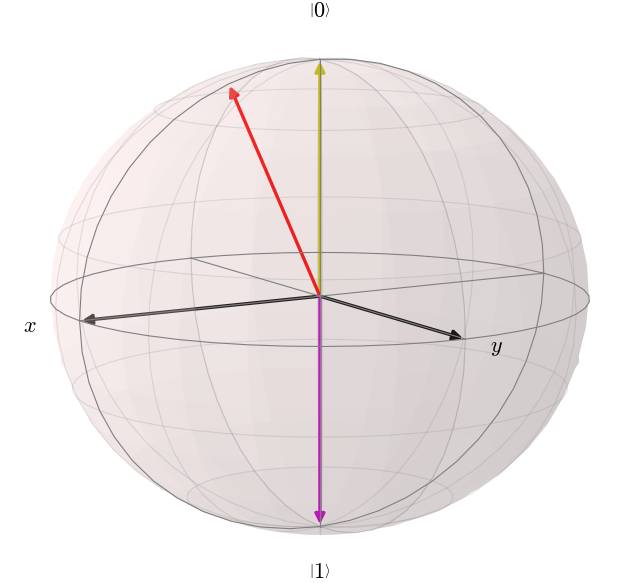
\includegraphics[scale=0.5]{img/bloch7over8.png}
       \caption{\label{img:7over8} Visualization of the second input qubit state $e^{-i\frac{\pi}{16}}\big[0.98079\ket{0} + 0.19509\ket{1}\big]$ coloured red on the Bloch sphere. The first training vector \0 is shown in yellow and the second training vector \1 is shown in purple.}
\end{figure}

The obtained simulation results after 1000 runs for both Bloch vectors from input data set II are shown in Table~\ref{tab:blochresults}. The theoretically predicted probabilities are marked with asterisks and are always displayed on top of the corresponding simulation result. Comparing these values shows strong agreement between prediction and simulation implying that 1000 simulation runs suffice to retrieve the expected probability distributions.

\begin{table}[H]
\begin{tabular}{| C{0.5cm} | C{2.7cm} |C{1.7cm} | C{1.7cm} | C{1.7cm} |C{1.8cm}| C{1.8cm}|}
      %\toprule
      ID & Qubit state  & $Prob(CM)$ & $Prob$ $(\ket{c} = \ket{0})$ & $Prob$ $(\ket{c} = \ket{1})$ & Expected class & Algorithm output\\
      \midrule
        1 & $e^{-i\frac{\pi}{8}}\big[0.92388\ket{0} + 0.38268\ket{1}\big]$ & \begin{tabular}{c} 0.8266* \\\midrule 0.8050 \end{tabular} & \begin{tabular}{c} 0.5818* \\\midrule 0.5863 \end{tabular} & \begin{tabular}{c} 0.4182* \\\midrule 0.4137 \end{tabular} & $\ket{0}$ (yellow) & $\ket{0}$ (yellow)\\\midrule
        
       2 & $e^{-i\frac{\pi}{16}}\big[0.98079\ket{0} + 0.19509\ket{1}\big]$ & \begin{tabular}{c} 0.7940* \\\midrule 0.7710 \end{tabular} & \begin{tabular}{c} 0.6237* \\\midrule 0.6420 \end{tabular} & \begin{tabular}{c} 0.3763* \\\midrule 0.3580 \end{tabular} & $\ket{0}$ (yellow) & $\ket{0}$ (yellow)\\\midrule
      \bottomrule
    \end{tabular}
    \caption{\label{tab:blochresults} Classification results for two qubit states after 1000 runs. Input state with ID=1 was defined in Table~\ref{tab:inputvectors} and qubit state with ID=2 was defined in Section~\ref{subsubsec:simulationamplitudeKNN}. Trained with training set defined in Table~\ref{tab:trainingset} consisting of the \0 and \1 qubit states. Theoretical predictions (marked with asterisks) on top, simulation results at the bottom.}
\end{table}

Both input qubit states were correctly classified as \0 (yellow vector in Fig.~\ref{img:3over4} and Fig.~\ref{fig:7over8}) as expected since both qubit states lie within the upper half of the Bloch sphere. The input qubit state with ID=2 has a slightly higher probability of being classified as \0 than the qubit state with ID=1. This is expected since the state with ID=2 is closer to the training state \0 on the Bloch sphere than the state with ID=1. 	

In conclusion, using the small input data set II the amplitude-based kNN algorithm has achieved 100\% accuracy. However, since only two Bloch vectors were considered this number should not be taken too seriously but rather be seen as a small test bench for the amplitude-based kNN algorithm. All in all, the main purpose of this simulation was to show that the amplitude-based kNN algorithm would have performed as expected when an implementation with IBM's quantum computer would have been feasible.

The classification of Bloch vectors considered in this section only made use of one qubit for each training and input vector. Since one qubit can only be in a superposition of maximally two states (e.g. the \0 and \1 state) only two amplitudes, e.g. one for the \0 and one for the \1 state, are available for data encoding. This was deliberately chosen since it made it relatively easy to construct the initial quantum state (Equ.~\ref{equ:ampinitial}) required for the amplitude-based kNN algorithm. The next section will increase the number of qubits used to encode each training and input vector and will describe how the simulated amplitude-based kNN algorithm can be used to classify different Gaussian distributions.

\subsubsection{Classification of Gaussian distributions}
\label{subsubsubsec:classificationblochvectors}

Section~\ref{subsubsec:classicaldataamplitudes} introduced the idea of encoding classical data into the $2^n$ amplitudes of a quantum state with $n$ qubits leading to exponential data compression compared to classical computers. Initializing arbitrary amplitude distributions is still actively researched and as discussed in Section~\ref{subsubsec:classicaldataamplitudes} requires the use of non-trivial quantum algorithms. However, this section will demonstrate and use the fact that it is relatively easy to initialize Gaussian amplitude distributions.

Consider the following classical probability vector $w$ with eight entries representing a discrete Gaussian distribution:

\begin{equation}
w = \colvec{0.58566\\0.11434\\0.11434\\0.022322\\0.11434\\0.022322\\0.022322\\0.0043579}
\end{equation}

The goal is to initialize an amplitude distribution of a multi-qubit system such that it represents the classical vector $w$. Since $w$ has eight entries the multi-qubit system needs to consist of three qubits giving rise to $2^3=8$ amplitudes. Thus, the desired quantum memory state $\ket{w}$ representing the classical vector $w$ should be of the form:

\begin{align}
\label{equ:desiredmemorystate}
\ket{w} = \quad &0.58566 \ket{000} + 0.11434 \ket{001} + 0.11434 \ket{010} +
0.02232 \ket{011}\notag\\
&+ 0.11434 \ket{100} + 0.02232 \ket{101} + + 0.02232 \ket{110} 
+ 0.00436 \ket{111}
\end{align}

Knowing that the classical vector $w$ is Gaussian-distributed it follows that the amplitudes of $\ket{w}$ are also Gaussian-distributed which will become important later. To initialize the state $\ket{w}$ a suitable quantum gate is required. For this purpose, the idea of a coin operator can be borrowed from the theory of quantum random walks (CITATION). Such a coin operator can be used as a quantum gate to initialize a Gaussian distribution centered around a chosen binary qubit pattern as will be shown later. For this purpose, the coin gate, denoted $C$, will be defined as the following unitary matrix:

\begin{equation}
C(\delta) = \begin{pmatrix}
\sqrt{\delta} & 1-\sqrt{\delta} \\
1-\sqrt{\delta} & -\sqrt{\delta}
\end{pmatrix}
\end{equation}

where $0 \leq \delta \leq 1$. The action of $C(\delta)$ on a quantum state needs to be analyzed to understand how it can be used to create Gaussian-distributed quantum states and how the parameter $\delta$ influences the shape of these distributions. For example, acting $C(\delta)$ on each individual qubit in the three-qubit state $\ket{000}$ yields:

\begin{align}
&(C(\delta) \otimes C(\delta) \otimes C(\delta)) \ket{000} = C(\delta)\ket{0} \otimes C(\delta)\ket{0} \otimes C(\delta)\ket{0}\notag\\
&\equiv \begin{pmatrix}
\sqrt{\delta} & 1-\sqrt{\delta} \\
1-\sqrt{\delta} & -\sqrt{\delta}
\end{pmatrix} \colvec{1\\0} \otimes \begin{pmatrix}
\sqrt{\delta} & 1-\sqrt{\delta} \\
1-\sqrt{\delta} & -\sqrt{\delta}
\end{pmatrix} \colvec{1\\0} \otimes \begin{pmatrix}
\sqrt{\delta} & 1-\sqrt{\delta} \\
1-\sqrt{\delta} & -\sqrt{\delta}
\end{pmatrix} \colvec{1\\0}\notag\\
&= \colvec{\sqrt{\delta}\\1-\sqrt{\delta}} \otimes \colvec{\sqrt{\delta}\\1-\sqrt{\delta}} \otimes \colvec{\sqrt{\delta}\\1-\sqrt{\delta}}\notag\\
&= \colvec{\sqrt{\delta}*\colvec{\sqrt{\delta}\\1-\sqrt{\delta}}\\(1-\sqrt{\delta})*\colvec{\sqrt{\delta}\\1-\sqrt{\delta}}} \otimes \colvec{\sqrt{\delta}\\1-\sqrt{\delta}}\notag\\
&= \colvec{\delta\\\sqrt{\delta}-\delta\\\sqrt{\delta}-\delta\\1-2\sqrt{\delta}+\delta} \otimes \colvec{\sqrt{\delta}\\1-\sqrt{\delta}}\notag\\
\label{equ:deltatensor}
&= \colvec{\delta\sqrt{\delta}\\\delta-\delta\sqrt{\delta}\\\delta-\delta\sqrt{\delta}\\\sqrt{\delta}(\delta+1)-2\delta\\\delta-\delta\sqrt{\delta}\\\sqrt{\delta}(\delta+1)-2\delta\\\sqrt{\delta}(\delta+1)-2\delta\\-\sqrt{\delta}(3+\delta)+1+3\delta}
\end{align}

When choosing $\delta = 0.7$, the last expression in Equ.~\ref{equ:deltatensor} is equal to the desired quantum memory state $\ket{w}$ defined in Equ.~\ref{equ:desiredmemorystate}:

\begin{align}
\label{equ:deltatensorsubbed}
\ket{w} &= \colvec{0.58566\\0.11434\\0.11434\\0.022322\\0.11434\\0.022322\\0.022322\\0.0043579}\notag\\
&\equiv 0.58566 \ket{000} + 0.11434 \ket{001} + 0.11434 \ket{010} +
0.02232 \ket{011}\notag\\
&\quad \quad + 0.11434 \ket{100} + 0.02232 \ket{101} + + 0.02232 \ket{110} 
+ 0.00436 \ket{111}
\end{align}

Thus, it was shown that acting $C(0.7)$ on each qubit in the state $\ket{000}$ yields the desired quantum memory state $\ket{w}$. Since the amplitudes of $\ket{w}$ represent a discretized Gaussian distribution, it was shown that the coin gate $C(\delta)$ can indeed be used to generate Gaussian amplitude distributions. 

Keeping in mind that $\ket{w}$ resulted from the action of $(C(0.7) \otimes C(0.7) \otimes C(0.7))$ onto the $\ket{000}$ state and important pattern is observed when calculating the Hamming distances between $\ket{000}$ and all eight possible three qubit states. Firstly, the state $\ket{000}$ has a Hamming distance of zero relative to itself and has the highest amplitude of 0.58566. Secondly, $\ket{100}$, $\ket{010}$ and $\ket{001}$ all have amplitudes of 0.11434 and a Hamming distance of one with respect to $\ket{000}$. Thirdly, $\ket{110}$, $\ket{011}$ and $\ket{101}$ have amplitudes of 0.02232 and a Hamming distance of two compared to $\ket{000}$. Lastly, $\ket{111}$ has a Hamming distance of three with respect to $\ket{000}$ and an amplitude of 0.00436. Hence, the amplitudes are always equal for equal Hamming distances and decrease with increasing Hamming distance.

To visualise the Gaussian distribution represented by $\ket{w}$, one simply needs to plot amplitudes against Hamming distances and mirror the resulting plot with respect to the vertical line connecting the horizontal zero value  with the data point representing the highest amplitude. The corresponding plot is given in Fig.~\ref{fig:gaussdeltaplot1} and clearly shows a discrete Gaussian distribution centered around the binary qubit pattern with Hamming distance zero: in this case $\ket{000}$. It follows that applying the coin gate $C(0.7)$ to each qubit in an $n$-qubit systems $\ket{q_1,q_2,...,q_n}$ yields a similar discretized Gaussian distribution centered around the binary qubit pattern $\ket{q_1,q_2,...,q_n}$.
%redefine the Hamming distance between $\ket{100}$ and $\ket{000}$ to be -1 instead of 1 and the Hamming distance between $ket{110}$ and $\ket{000}$ to be -2 instead of 2. Furthermore, suppose one can add a ninth entry to $\ket{w}$ by duplicating the entry for state $\ket{111}$. Define the new duplicate entry of $\ket{111}$ to have a Hamming distance of -3 instead of 3. When plotting the Hamming distances against the amplitudes of this new artificial vector representation of $\ket{w}$ a discrete Gaussian distribution can be observed. The corresponding plot in Fig.~\ref{fig:gaussdeltaplot1} illustrates this clearly.

\begin{figure}[H]
\centering
    \begin{tikzpicture}[scale=1]
\begin{axis}[xlabel={Hamming distance},ylabel={Amplitude},
				xtick=data,xticklabel style={align=center},xticklabels={3,2,1,0,1,2,3}]
				
				%xticklabels={{3\\($\ket{111}$)},{2\\($\ket{011}$)\\($\ket{110}$)\\($\ket{101}$)},{1\\($\ket{100}$)\\($\ket{010}$)\\($\ket{001}$)},{0\\($\ket{000}$)},{1\\($\ket{100}$)\\($\ket{010}$)\\($\ket{001}$)},{2\\($\ket{011}$)\\($\ket{110}$)\\($\ket{101}$)},{3\\($\ket{111}$)}}]

% Graph column 0 versus column 1
\addplot table[x index=1,y index=0,col sep=comma] {gauss2.dat};
\addlegendentry{$\delta = 0.7$}% y index+1 since humans count from 1

\end{axis}
\end{tikzpicture}
\caption{Plot visualizing the discrete Gaussian distribution of $\ket{w}$ resulting from acting coin gate $C$ with $\delta =0.7$ on each qubit in state $\ket{000}$. Amplitudes of quantum state $\ket{w}$ (Equ.~\ref{equ:desiredmemorystate}) are plotted against the Hamming distances between binary pattern $\ket{000}$ and all eight binary three-qubit pattern. The plot was mirrored with respect to the vertical line connecting the horizontal zero value with the data point representing the highest amplitude.}
\label{fig:gaussdeltaplot1}
  \end{figure}
  
The observed pattern within the amplitudes can be generalized using Equ.~\ref{equ:deltatensor}: Acting the coin gate $C(\delta)$ on each qubit in the three-qubit state $\ket{000}$ will result in a discretized Gaussian distribution centered around $\ket{000}$ with the following amplitudes dependent on the Hamming distance with respect to state $\ket{000}$: state $\ket{000}$ with Hamming distance zero will have the largest amplitude of $\delta\sqrt{\delta}$, states with Hamming distance one have amplitudes equal to $\delta-\delta\sqrt{\delta}$, states with Hamming distance two have amplitudes equal to $\sqrt{\delta}(\delta+1)-2\delta$ and the state $\ket{111}$ with the largest Hamming distance of three has the smallest amplitude of $-\sqrt{\delta}(3+\delta)+1+3\delta$.
  
A useful tool for visualizing Hamming distances between three-qubit patterns is a three-dimensional cube as shown in Fig.~\ref{img:cubenoprobs}. On that cube, adjacent qubit patterns have a Hamming distance (HD) of one and the Hamming distance increases by one with every additional corner. For example, the qubit state $\ket{100}$ is adjacent to $\ket{110}$ since they only differ in one qubit ($HD=1$). Moving one more corner yields the state $\ket{111}$ or $\ket{010}$ which both have a Hamming distance of two when compared to $\ket{100}$.

\begin{figure}[!ht]
       \centering
       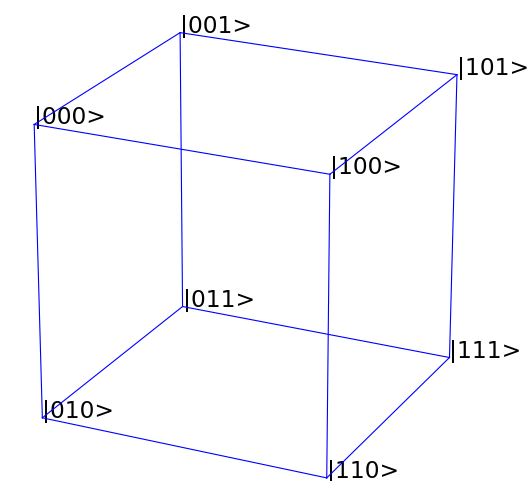
\includegraphics[width=0.5\textwidth]{img/cubewithoutprobs.png}
       \caption{\label{img:cubenoprobs} Visualizing Hamming distances on a three-dimensional cube. The Hamming distance between two binary qubit patterns is given by the shortest path on the edges of the cube between them. Thereby, the Hamming distance increases by one for every corner.}
\end{figure}

This cube can be used as another way of visualizing the action of the coin gate $C(0.7)$ on each qubit in the e.g. $\ket{000}$ state. Before applying the $C$ gates the qubit state is $\ket{000}$ with an amplitude of 1.0 shown in Fig.~\ref{img:cubeoneprob} wherein amplitude is denoted by $a$.
  
\begin{figure}[H]
       \centering
       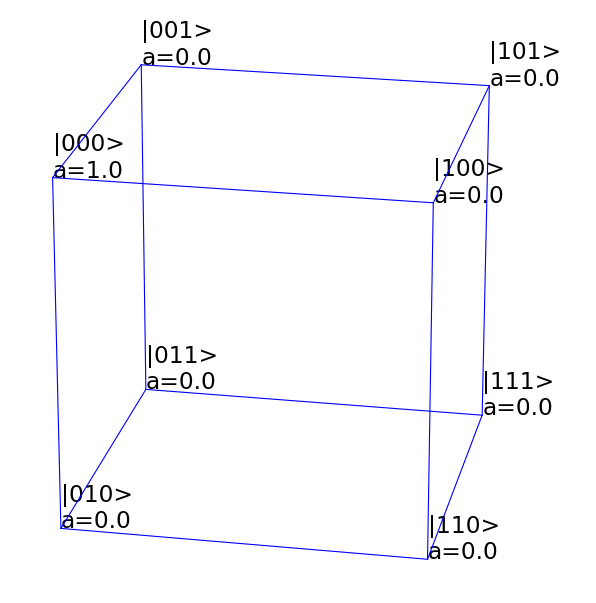
\includegraphics[width=0.5\textwidth]{img/cubeoneprob.png}
       \caption{\label{img:cubeoneprob} The qubit state $\ket{000}$ with amplitude ($a$) of 1.0 visualized on a three-dimensional cube representing the Hamming distances between binary qubit patterns.}
\end{figure}

Applying the coin gate $C$ to the first qubit redistributes the amplitudes between the $\ket{000}$ and $\ket{100}$ state which is visualized in Fig.~\ref{img:cubediffused1} below.

\begin{figure}[H]
       \centering
       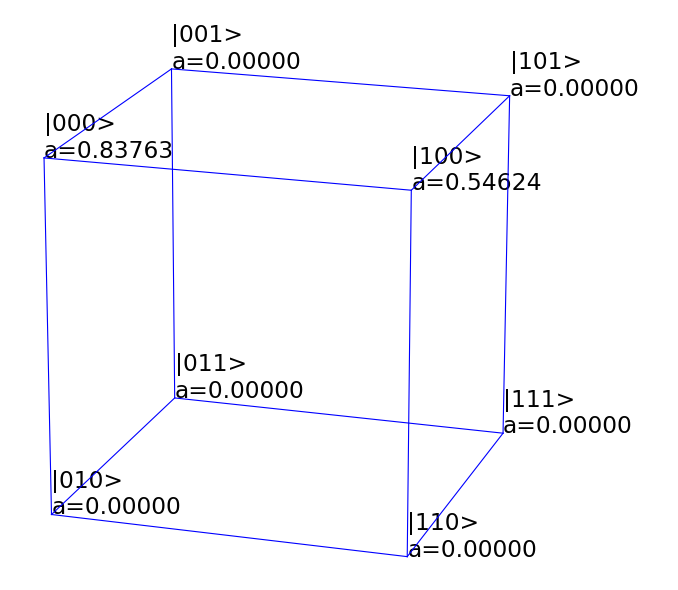
\includegraphics[width=0.5\textwidth]{img/cube_diffused1.png}
       \caption{\label{img:cubediffused1} Visualization of the amplitude distribution over all three-qubit states after application of coin gate $C$ to the first qubit of the state $\ket{000}$.}
\end{figure}

Fig.~\ref{img:cubediffused2} illustrates the amplitude distribution after application of $C$ gates to the first and second qubit in the state $\ket{000}$. It can be seen that only four out of eight three-qubit states have non-zero amplitudes at this point. With the application of the third $C$ gate to the third qubit in $\ket{000}$ all eight qubit patterns have non-zero amplitudes and the quantum state $\ket{w}$ from Equ.~\ref{equ:desiredmemorystate} is obtained. Fig.~\ref{img:cubediffused3} shows this final quantum superposition representing a discrete Gaussian distribution over a three-dimensional cube based on Hamming distances.

In this example, Fig.~\ref{img:cubediffused1}, ~\ref{img:cubediffused2} and \ref{img:cubediffused3} visually demonstrate a stepwise diffusion of the initial amplitude of 1.0 from $\ket{000}$ over all eight three-qubit patterns on the cube.

\begin{minipage}[c]{.5\textwidth}
       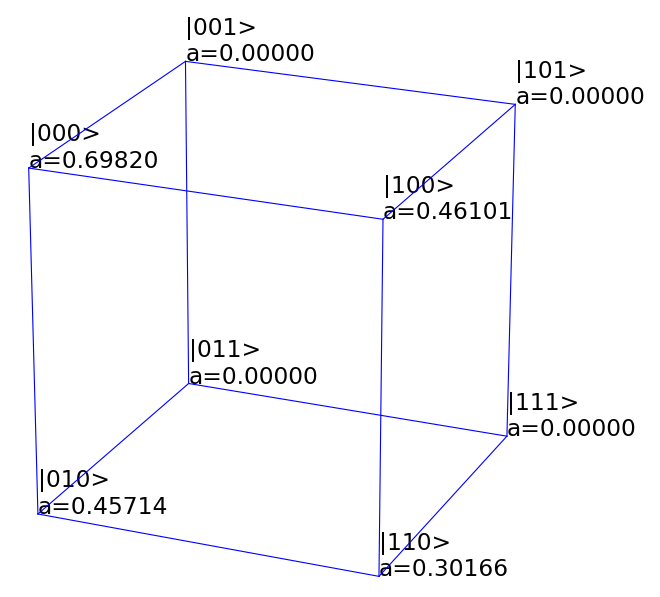
\includegraphics[width=1\textwidth]{img/cube_diffused2.png}
       \captionsetup{justification=raggedright, singlelinecheck=false}
       \captionof{figure}{\label{img:cubediffused2} Visualization of the amplitude distribution over all three-qubit states after application of coin gate $C$ to the first two \\qubits in the state $\ket{000}$.}
\end{minipage}%%%%%
\begin{minipage}[c]{.5\textwidth}
       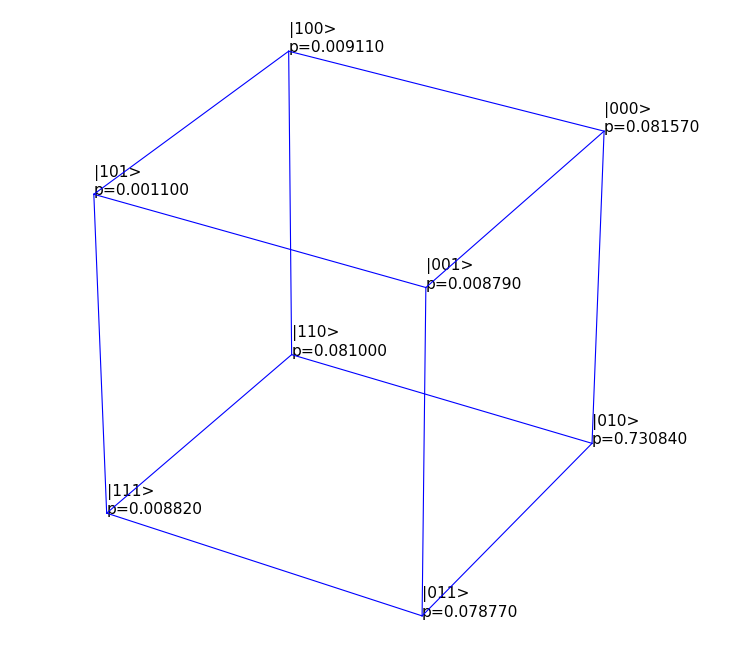
\includegraphics[width=1\textwidth]{img/cube_diffused.png} \captionsetup{justification=raggedright, singlelinecheck=false}
       \captionof{figure}{\label{img:cubediffused3} Final amplitude distribution over all three-qubit states after application of coin gate $C$ to each qubit in the state $\ket{000}$ visualized on a three-dimensional cube.}
\end{minipage}


\begin{figure}[H]
\centering
    \begin{tikzpicture}[scale=1.3]
\begin{axis}[xlabel={Hamming distance},ylabel={Probability},xtick=data,xticklabels={4,3,2,1,0,1,2,3,4}]

% Graph column 0 versus column 1
\addplot table[x index=1,y index=0,col sep=comma] {gauss1.dat};
\addlegendentry{$\delta = 0.9$}% y index+1 since humans count from 1

% Graph column 2 versus column 1 
\addplot table[x index=1,y index=2,col sep=comma] {gauss1.dat};
\addlegendentry{$\delta = 0.8$}

% Graph column 3 versus column 1    
\addplot table[x index=1,y index=3,col sep=comma] {gauss1.dat};
\addlegendentry{$\delta = 0.7$}

% Graph column 4 versus column 1    
\addplot table[x index=1,y index=4,col sep=comma] {gauss1.dat};
\addlegendentry{$\delta = 0.6$}

% Graph column 5 versus column 1   
\addplot table[x index=1,y index=5,col sep=comma] {gauss1.dat};
\addlegendentry{$\delta = 0.5$}

\end{axis}
\end{tikzpicture}
\caption{Gaussian distributions}
\label{fig:gaussdeltaplot2}
  \end{figure}

This way of visualizing HDs can be extended to the 16 binary patterns made by four qubits that can be visualized on a 4-D cube, also called tesseract, as illustrated in Fig.~\ref{img:hypercubenoprobs}.

\begin{figure}[!ht]
       \centering
       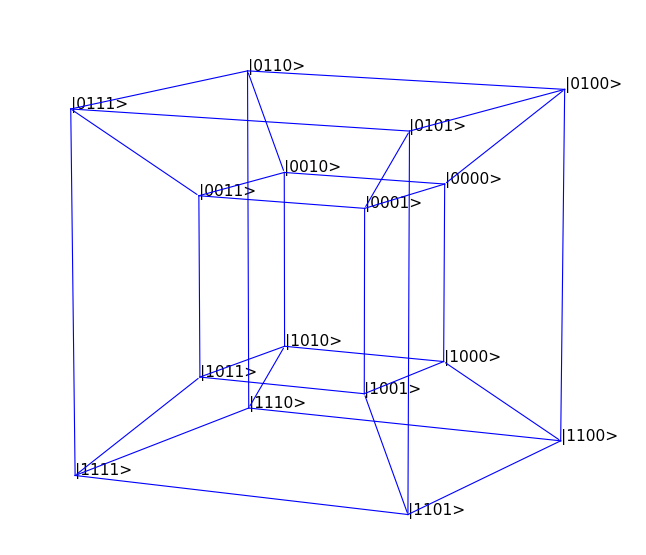
\includegraphics[width=0.5\textwidth]{img/hypercubewithoutprobs.png}
       \caption{\label{img:hypercubenoprobs} Visualizing Hamming distances on a 4-D cube (tesseract)}
\end{figure}


Initializing gaussian distributed quantum states and classifying gaussian distributions by means of the Hellinger distance.

\begin{redbox}
\textbf{Definition: Hellinger distance}\\
\newline
The Hellinger distance is a distance metric used to quantify the difference between any two probability distributions. In the case of continuous probability distributions it is defined using the Hellinger integral first proposed by \citeA{hellinger1909neue}. However, since the $2^n$ amplitudes of an $n$-qubit system will always constitute a discrete probability distribution only the Hellinger distance for discrete distributions will be introduced.\\
\newline
The Hellinger distance between two probability distributions $R = (r_1,...,r_j)$ and $T = (t_1,...,t_j)$ is defined as:

\begin{equation}
\label{equ:hellingerdistance}
H(R,T) = \frac{1}{\sqrt{2}}\sqrt{\sum_{i=1}^j (\sqrt{r_i} - \sqrt{t_i})^2}
\end{equation}

and can be rewritten in terms of the Euclidean distance between the square root vectors $\sqrt{R}$ and $\sqrt{T}$:

\begin{equation}
H(R,T) = \frac{1}{\sqrt{2}} \mid\mid\sqrt{R} - \sqrt{T}\mid\mid_2
\end{equation}
\end{redbox}

\begin{equation}
Prob(\ket{c^m} = \ket{1(\textcolor{purple}{B})})= \sum_{m \mid c^m=1(\textcolor{purple}{B})} 1 - \frac{1}{4M} \sum_{i=1}^N \mid \textcolor{red}{x_i} - \textcolor{purple}{t^m_i} \mid ^2
\end{equation}

Hence, if $x_i = \sqrt{w_i}$ where $w_i$ is the i\textsuperscript{th} element of the classical probability vector $w$ the aKNN algorithm classification outcome is dependent on the squared Hellinger distance. This can be obtained by squaring Equ.~\ref{equ:hellingerdistance} yielding:
\begin{equation}
\label{equ:squaredhellingerdistance}
H^2(R,T) = \frac{1}{\sqrt{2}}\sum_{i=1}^j (\sqrt{r_i} - \sqrt{t_i})^2
\end{equation}





